\documentclass[]{article}
\usepackage{lmodern}
\usepackage{amssymb,amsmath}
\usepackage{ifxetex,ifluatex}
\usepackage{fixltx2e} % provides \textsubscript
\ifnum 0\ifxetex 1\fi\ifluatex 1\fi=0 % if pdftex
  \usepackage[T1]{fontenc}
  \usepackage[utf8]{inputenc}
\else % if luatex or xelatex
  \ifxetex
    \usepackage{mathspec}
  \else
    \usepackage{fontspec}
  \fi
  \defaultfontfeatures{Ligatures=TeX,Scale=MatchLowercase}
\fi
% use upquote if available, for straight quotes in verbatim environments
\IfFileExists{upquote.sty}{\usepackage{upquote}}{}
% use microtype if available
\IfFileExists{microtype.sty}{%
\usepackage{microtype}
\UseMicrotypeSet[protrusion]{basicmath} % disable protrusion for tt fonts
}{}
\usepackage[margin=1in]{geometry}
\usepackage{hyperref}
\hypersetup{unicode=true,
            pdftitle={Figure Paper},
            pdfauthor={Valeria Policastro},
            pdfborder={0 0 0},
            breaklinks=true}
\urlstyle{same}  % don't use monospace font for urls
\usepackage{color}
\usepackage{fancyvrb}
\newcommand{\VerbBar}{|}
\newcommand{\VERB}{\Verb[commandchars=\\\{\}]}
\DefineVerbatimEnvironment{Highlighting}{Verbatim}{commandchars=\\\{\}}
% Add ',fontsize=\small' for more characters per line
\usepackage{framed}
\definecolor{shadecolor}{RGB}{248,248,248}
\newenvironment{Shaded}{\begin{snugshade}}{\end{snugshade}}
\newcommand{\KeywordTok}[1]{\textcolor[rgb]{0.13,0.29,0.53}{\textbf{#1}}}
\newcommand{\DataTypeTok}[1]{\textcolor[rgb]{0.13,0.29,0.53}{#1}}
\newcommand{\DecValTok}[1]{\textcolor[rgb]{0.00,0.00,0.81}{#1}}
\newcommand{\BaseNTok}[1]{\textcolor[rgb]{0.00,0.00,0.81}{#1}}
\newcommand{\FloatTok}[1]{\textcolor[rgb]{0.00,0.00,0.81}{#1}}
\newcommand{\ConstantTok}[1]{\textcolor[rgb]{0.00,0.00,0.00}{#1}}
\newcommand{\CharTok}[1]{\textcolor[rgb]{0.31,0.60,0.02}{#1}}
\newcommand{\SpecialCharTok}[1]{\textcolor[rgb]{0.00,0.00,0.00}{#1}}
\newcommand{\StringTok}[1]{\textcolor[rgb]{0.31,0.60,0.02}{#1}}
\newcommand{\VerbatimStringTok}[1]{\textcolor[rgb]{0.31,0.60,0.02}{#1}}
\newcommand{\SpecialStringTok}[1]{\textcolor[rgb]{0.31,0.60,0.02}{#1}}
\newcommand{\ImportTok}[1]{#1}
\newcommand{\CommentTok}[1]{\textcolor[rgb]{0.56,0.35,0.01}{\textit{#1}}}
\newcommand{\DocumentationTok}[1]{\textcolor[rgb]{0.56,0.35,0.01}{\textbf{\textit{#1}}}}
\newcommand{\AnnotationTok}[1]{\textcolor[rgb]{0.56,0.35,0.01}{\textbf{\textit{#1}}}}
\newcommand{\CommentVarTok}[1]{\textcolor[rgb]{0.56,0.35,0.01}{\textbf{\textit{#1}}}}
\newcommand{\OtherTok}[1]{\textcolor[rgb]{0.56,0.35,0.01}{#1}}
\newcommand{\FunctionTok}[1]{\textcolor[rgb]{0.00,0.00,0.00}{#1}}
\newcommand{\VariableTok}[1]{\textcolor[rgb]{0.00,0.00,0.00}{#1}}
\newcommand{\ControlFlowTok}[1]{\textcolor[rgb]{0.13,0.29,0.53}{\textbf{#1}}}
\newcommand{\OperatorTok}[1]{\textcolor[rgb]{0.81,0.36,0.00}{\textbf{#1}}}
\newcommand{\BuiltInTok}[1]{#1}
\newcommand{\ExtensionTok}[1]{#1}
\newcommand{\PreprocessorTok}[1]{\textcolor[rgb]{0.56,0.35,0.01}{\textit{#1}}}
\newcommand{\AttributeTok}[1]{\textcolor[rgb]{0.77,0.63,0.00}{#1}}
\newcommand{\RegionMarkerTok}[1]{#1}
\newcommand{\InformationTok}[1]{\textcolor[rgb]{0.56,0.35,0.01}{\textbf{\textit{#1}}}}
\newcommand{\WarningTok}[1]{\textcolor[rgb]{0.56,0.35,0.01}{\textbf{\textit{#1}}}}
\newcommand{\AlertTok}[1]{\textcolor[rgb]{0.94,0.16,0.16}{#1}}
\newcommand{\ErrorTok}[1]{\textcolor[rgb]{0.64,0.00,0.00}{\textbf{#1}}}
\newcommand{\NormalTok}[1]{#1}
\usepackage{graphicx,grffile}
\makeatletter
\def\maxwidth{\ifdim\Gin@nat@width>\linewidth\linewidth\else\Gin@nat@width\fi}
\def\maxheight{\ifdim\Gin@nat@height>\textheight\textheight\else\Gin@nat@height\fi}
\makeatother
% Scale images if necessary, so that they will not overflow the page
% margins by default, and it is still possible to overwrite the defaults
% using explicit options in \includegraphics[width, height, ...]{}
\setkeys{Gin}{width=\maxwidth,height=\maxheight,keepaspectratio}
\IfFileExists{parskip.sty}{%
\usepackage{parskip}
}{% else
\setlength{\parindent}{0pt}
\setlength{\parskip}{6pt plus 2pt minus 1pt}
}
\setlength{\emergencystretch}{3em}  % prevent overfull lines
\providecommand{\tightlist}{%
  \setlength{\itemsep}{0pt}\setlength{\parskip}{0pt}}
\setcounter{secnumdepth}{0}
% Redefines (sub)paragraphs to behave more like sections
\ifx\paragraph\undefined\else
\let\oldparagraph\paragraph
\renewcommand{\paragraph}[1]{\oldparagraph{#1}\mbox{}}
\fi
\ifx\subparagraph\undefined\else
\let\oldsubparagraph\subparagraph
\renewcommand{\subparagraph}[1]{\oldsubparagraph{#1}\mbox{}}
\fi

%%% Use protect on footnotes to avoid problems with footnotes in titles
\let\rmarkdownfootnote\footnote%
\def\footnote{\protect\rmarkdownfootnote}

%%% Change title format to be more compact
\usepackage{titling}

% Create subtitle command for use in maketitle
\providecommand{\subtitle}[1]{
  \posttitle{
    \begin{center}\large#1\end{center}
    }
}

\setlength{\droptitle}{-2em}

  \title{Figure Paper}
    \pretitle{\vspace{\droptitle}\centering\huge}
  \posttitle{\par}
    \author{Valeria Policastro}
    \preauthor{\centering\large\emph}
  \postauthor{\par}
      \predate{\centering\large\emph}
  \postdate{\par}
    \date{20 settembre 2019}


\begin{document}
\maketitle

\section{Fig.3 Plot of the two curves for the
robustness}\label{fig.3-plot-of-the-two-curves-for-the-robustness}

\begin{Shaded}
\begin{Highlighting}[]
\KeywordTok{library}\NormalTok{(}\StringTok{"cowplot"}\NormalTok{)}
\end{Highlighting}
\end{Shaded}

\begin{verbatim}
## Loading required package: ggplot2
\end{verbatim}

\begin{verbatim}
## 
## Attaching package: 'cowplot'
\end{verbatim}

\begin{verbatim}
## The following object is masked from 'package:ggplot2':
## 
##     ggsave
\end{verbatim}

\begin{Shaded}
\begin{Highlighting}[]
\KeywordTok{library}\NormalTok{(}\StringTok{"robin"}\NormalTok{)}
\end{Highlighting}
\end{Shaded}

\begin{verbatim}
## Loading required package: igraph
\end{verbatim}

\begin{verbatim}
## 
## Attaching package: 'igraph'
\end{verbatim}

\begin{verbatim}
## The following objects are masked from 'package:stats':
## 
##     decompose, spectrum
\end{verbatim}

\begin{verbatim}
## The following object is masked from 'package:base':
## 
##     union
\end{verbatim}

\begin{Shaded}
\begin{Highlighting}[]
\KeywordTok{library}\NormalTok{(}\StringTok{"gprege"}\NormalTok{)}
\end{Highlighting}
\end{Shaded}

\begin{verbatim}
## Loading required package: gptk
\end{verbatim}

\begin{verbatim}
## Loading required package: Matrix
\end{verbatim}

\begin{verbatim}
## Loading required package: fields
\end{verbatim}

\begin{verbatim}
## Loading required package: spam
\end{verbatim}

\begin{verbatim}
## Loading required package: dotCall64
\end{verbatim}

\begin{verbatim}
## Loading required package: grid
\end{verbatim}

\begin{verbatim}
## Spam version 2.2-2 (2019-03-07) is loaded.
## Type 'help( Spam)' or 'demo( spam)' for a short introduction 
## and overview of this package.
## Help for individual functions is also obtained by adding the
## suffix '.spam' to the function name, e.g. 'help( chol.spam)'.
\end{verbatim}

\begin{verbatim}
## 
## Attaching package: 'spam'
\end{verbatim}

\begin{verbatim}
## The following object is masked from 'package:Matrix':
## 
##     det
\end{verbatim}

\begin{verbatim}
## The following objects are masked from 'package:base':
## 
##     backsolve, forwardsolve
\end{verbatim}

\begin{verbatim}
## Loading required package: maps
\end{verbatim}

\begin{verbatim}
## See https://github.com/NCAR/Fields for
##  an extensive vignette, other supplements and source code
\end{verbatim}

\begin{Shaded}
\begin{Highlighting}[]
\NormalTok{my_file <-}\StringTok{ }\KeywordTok{system.file}\NormalTok{(}\StringTok{"example/football.gml"}\NormalTok{, }\DataTypeTok{package=}\StringTok{"robin"}\NormalTok{)}
\NormalTok{graph <-}\StringTok{ }\KeywordTok{prepGraph}\NormalTok{(}\DataTypeTok{file=}\NormalTok{my_file, }\DataTypeTok{file.format=}\StringTok{"gml"}\NormalTok{)}
\NormalTok{graphRandom <-}\StringTok{ }\KeywordTok{random}\NormalTok{(}\DataTypeTok{graph=}\NormalTok{graph)}
\NormalTok{proc <-}\StringTok{ }\KeywordTok{robinRobust}\NormalTok{(}\DataTypeTok{graph=}\NormalTok{graph, }\DataTypeTok{graphRandom=}\NormalTok{graphRandom, }\DataTypeTok{measure=}\StringTok{"vi"}\NormalTok{, }
                  \DataTypeTok{method=}\StringTok{"louvain"}\NormalTok{, }\DataTypeTok{type=}\StringTok{"independent"}\NormalTok{)}
\end{Highlighting}
\end{Shaded}

\begin{verbatim}
## [1] 31
## [1] 61
## [1] 92
## [1] 123
## [1] 153
## [1] 184
## [1] 215
## [1] 245
## [1] 276
## [1] 306
## [1] 337
## [1] 368
\end{verbatim}

\begin{Shaded}
\begin{Highlighting}[]
\KeywordTok{plotRobin}\NormalTok{(}\DataTypeTok{graph=}\NormalTok{graph, }\DataTypeTok{model1=}\NormalTok{proc}\OperatorTok{$}\NormalTok{Mean, }\DataTypeTok{model2=}\NormalTok{proc}\OperatorTok{$}\NormalTok{MeanRandom, }
\DataTypeTok{legend=}\KeywordTok{c}\NormalTok{(}\StringTok{"real data"}\NormalTok{, }\StringTok{"null model"}\NormalTok{), }\DataTypeTok{measure=}\StringTok{"vi"}\NormalTok{)}
\end{Highlighting}
\end{Shaded}

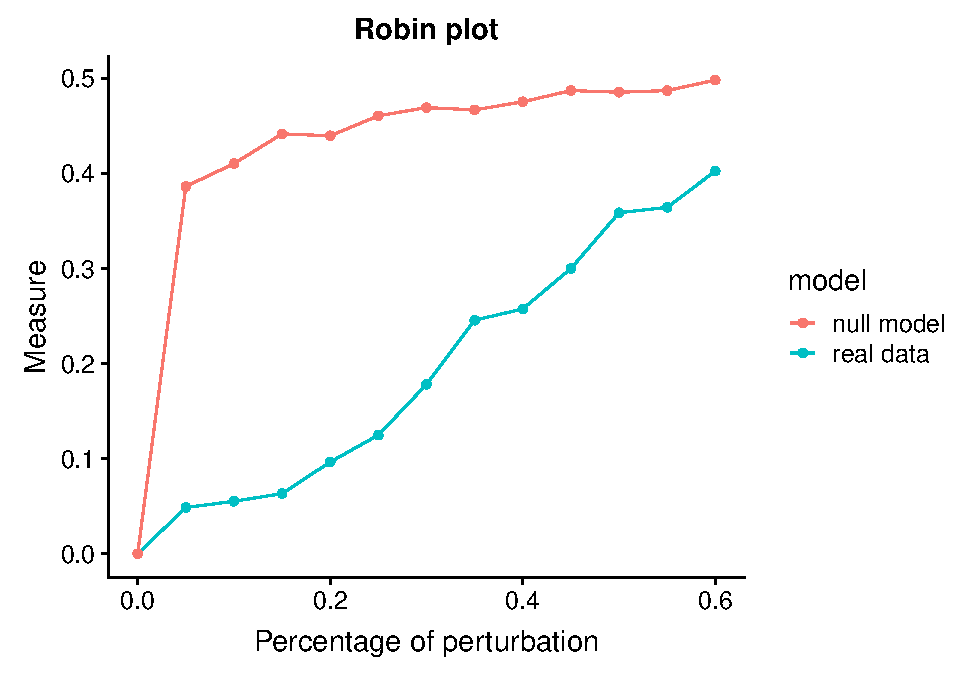
\includegraphics{Figure_Paper_files/figure-latex/unnamed-chunk-1-1.pdf}

\section{Fig.4 Plot for the comparison of the two
algorithms}\label{fig.4-plot-for-the-comparison-of-the-two-algorithms}

\begin{Shaded}
\begin{Highlighting}[]
\NormalTok{comp <-}\StringTok{ }\KeywordTok{robinCompare}\NormalTok{(}\DataTypeTok{graph=}\NormalTok{graph, }\DataTypeTok{method1=}\StringTok{"fastGreedy"}\NormalTok{,}
                \DataTypeTok{method2=}\StringTok{"louvain"}\NormalTok{, }\DataTypeTok{measure=}\StringTok{"vi"}\NormalTok{, }\DataTypeTok{type=}\StringTok{"independent"}\NormalTok{)}
\end{Highlighting}
\end{Shaded}

\begin{verbatim}
## [1] 31
## [1] 61
## [1] 92
## [1] 123
## [1] 153
## [1] 184
## [1] 215
## [1] 245
## [1] 276
## [1] 306
## [1] 337
## [1] 368
\end{verbatim}

\begin{Shaded}
\begin{Highlighting}[]
\KeywordTok{plotRobin}\NormalTok{(}\DataTypeTok{graph=}\NormalTok{graph, }\DataTypeTok{model1=}\NormalTok{comp}\OperatorTok{$}\NormalTok{Mean1, }\DataTypeTok{model2=}\NormalTok{comp}\OperatorTok{$}\NormalTok{Mean2, }\DataTypeTok{measure=}\StringTok{"vi"}\NormalTok{, }
\DataTypeTok{legend=}\KeywordTok{c}\NormalTok{(}\StringTok{"fastGreedy"}\NormalTok{, }\StringTok{"louvain"}\NormalTok{), }\DataTypeTok{title=}\StringTok{"FastGreedy vs Louvain"}\NormalTok{)}
\end{Highlighting}
\end{Shaded}

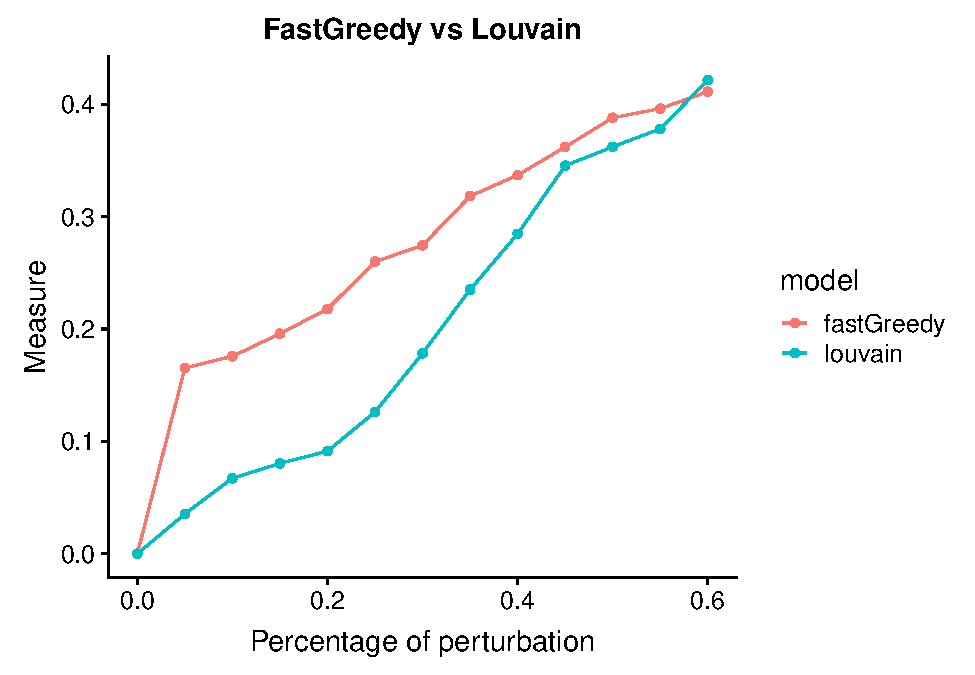
\includegraphics{Figure_Paper_files/figure-latex/unnamed-chunk-2-1.pdf}

\section{Fig.5 Functional Data Analysis
Test}\label{fig.5-functional-data-analysis-test}

\begin{Shaded}
\begin{Highlighting}[]
\KeywordTok{robinFDATest}\NormalTok{(}\DataTypeTok{graph=}\NormalTok{graph, }\DataTypeTok{model1=}\NormalTok{comp}\OperatorTok{$}\NormalTok{Mean1, }\DataTypeTok{model2=}\NormalTok{comp}\OperatorTok{$}\NormalTok{Mean2, }\DataTypeTok{measure=}\StringTok{"vi"}\NormalTok{)}
\end{Highlighting}
\end{Shaded}

\begin{verbatim}
## [1] "First step: basis expansion"
## Swapping 'y' and 'argvals', because 'y' is  simpler,
##   and 'argvals' should be;  now  dim(argvals) =  13 ;  dim(y) =  13 x 20 
## [1] "Second step: joint univariate tests"
## [1] "Third step: interval-wise combination and correction"
## [1] "creating the p-value matrix: end of row 2 out of 9"
## [1] "creating the p-value matrix: end of row 3 out of 9"
## [1] "creating the p-value matrix: end of row 4 out of 9"
## [1] "creating the p-value matrix: end of row 5 out of 9"
## [1] "creating the p-value matrix: end of row 6 out of 9"
## [1] "creating the p-value matrix: end of row 7 out of 9"
## [1] "creating the p-value matrix: end of row 8 out of 9"
## [1] "creating the p-value matrix: end of row 9 out of 9"
## [1] "Interval Testing Procedure completed"
\end{verbatim}

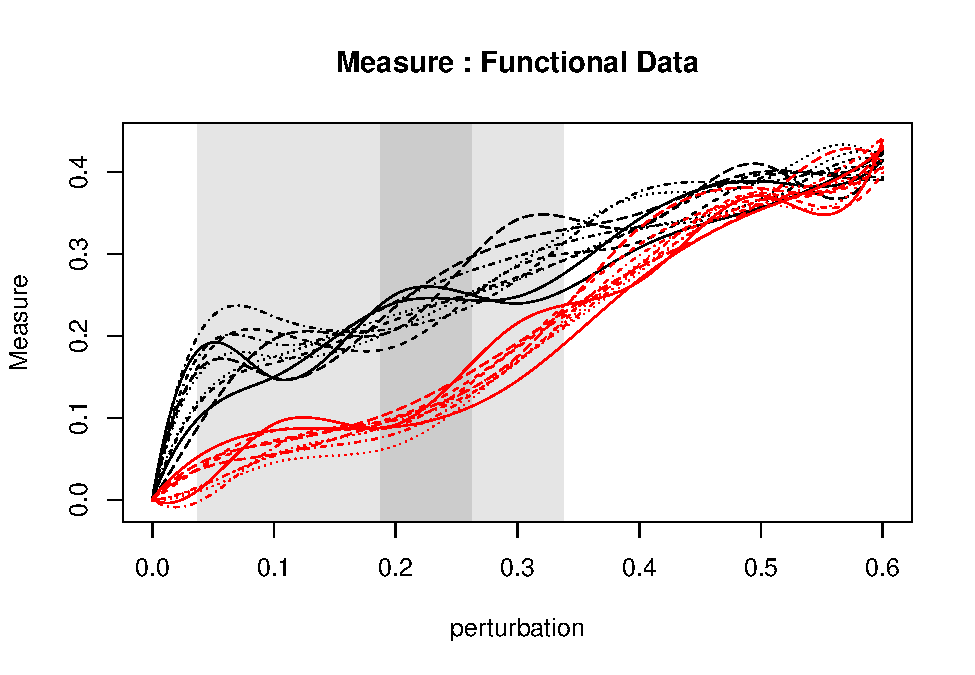
\includegraphics{Figure_Paper_files/figure-latex/unnamed-chunk-3-1.pdf}
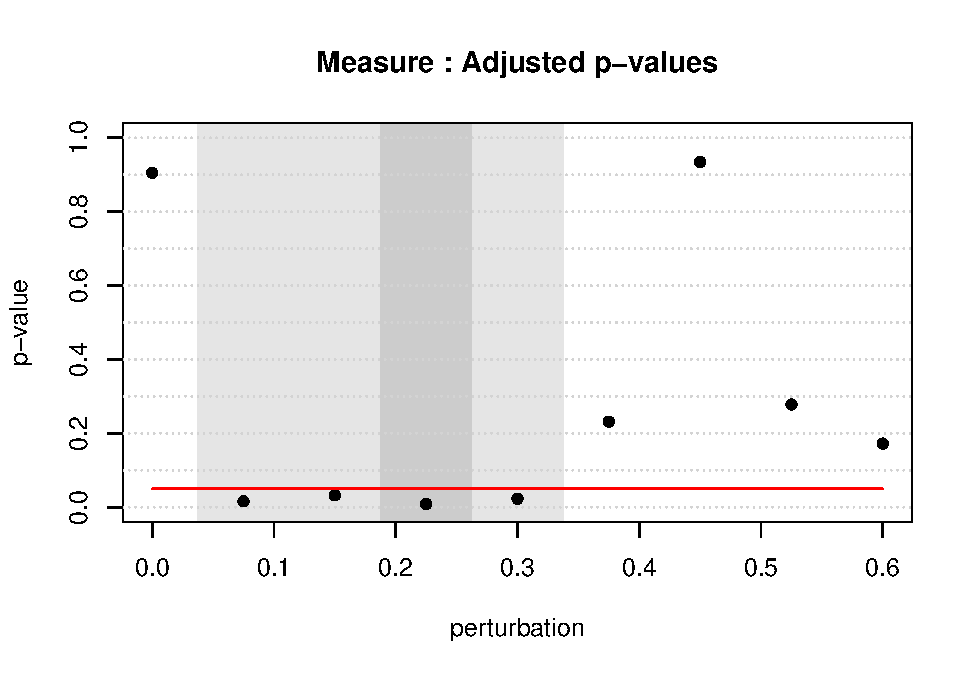
\includegraphics{Figure_Paper_files/figure-latex/unnamed-chunk-3-2.pdf}

\begin{verbatim}
## $ask
## [1] TRUE
\end{verbatim}

\section{Fig.6 VI measure for all
algorithms}\label{fig.6-vi-measure-for-all-algorithms}

\begin{Shaded}
\begin{Highlighting}[]
\CommentTok{#1}
\NormalTok{comp <-}\StringTok{ }\KeywordTok{robinCompare}\NormalTok{(}\DataTypeTok{graph=}\NormalTok{graph, }\DataTypeTok{method1=}\StringTok{"louvain"}\NormalTok{,}
                \DataTypeTok{method2=}\StringTok{"fastGreedy"}\NormalTok{, }\DataTypeTok{measure=}\StringTok{"vi"}\NormalTok{, }\DataTypeTok{type=}\StringTok{"independent"}\NormalTok{)}
\end{Highlighting}
\end{Shaded}

\begin{verbatim}
## [1] 31
## [1] 61
## [1] 92
## [1] 123
## [1] 153
## [1] 184
## [1] 215
## [1] 245
## [1] 276
## [1] 306
## [1] 337
## [1] 368
\end{verbatim}

\begin{Shaded}
\begin{Highlighting}[]
\KeywordTok{plotRobin}\NormalTok{(}\DataTypeTok{graph=}\NormalTok{graph, }\DataTypeTok{model1=}\NormalTok{comp}\OperatorTok{$}\NormalTok{Mean1, }\DataTypeTok{model2=}\NormalTok{comp}\OperatorTok{$}\NormalTok{Mean2, }\DataTypeTok{measure=}\StringTok{"vi"}\NormalTok{, }
\DataTypeTok{legend=}\KeywordTok{c}\NormalTok{(}\StringTok{"louvain"}\NormalTok{, }\StringTok{"fastGreedy"}\NormalTok{), }\DataTypeTok{title=}\StringTok{"Louvain vs FastGreedy"}\NormalTok{)}
\end{Highlighting}
\end{Shaded}

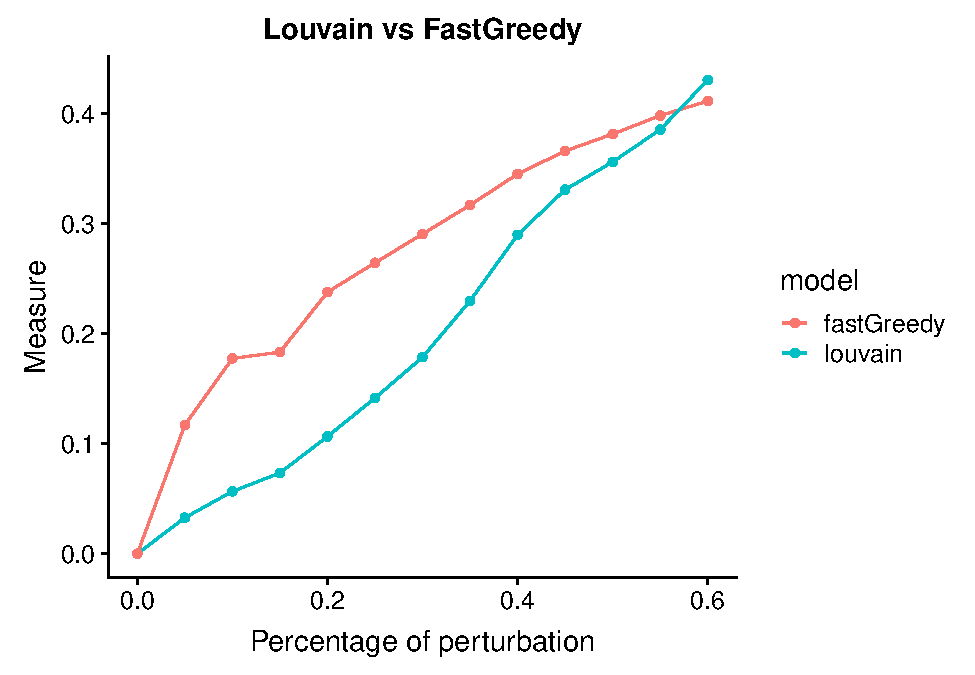
\includegraphics{Figure_Paper_files/figure-latex/unnamed-chunk-4-1.pdf}

\begin{Shaded}
\begin{Highlighting}[]
\CommentTok{#2}
\NormalTok{comp <-}\StringTok{ }\KeywordTok{robinCompare}\NormalTok{(}\DataTypeTok{graph=}\NormalTok{graph, }\DataTypeTok{method1=}\StringTok{"louvain"}\NormalTok{,}
                \DataTypeTok{method2=}\StringTok{"walktrap"}\NormalTok{, }\DataTypeTok{measure=}\StringTok{"vi"}\NormalTok{, }\DataTypeTok{type=}\StringTok{"independent"}\NormalTok{)}
\end{Highlighting}
\end{Shaded}

\begin{verbatim}
## [1] 31
## [1] 61
## [1] 92
## [1] 123
## [1] 153
## [1] 184
## [1] 215
## [1] 245
## [1] 276
## [1] 306
## [1] 337
## [1] 368
\end{verbatim}

\begin{Shaded}
\begin{Highlighting}[]
\KeywordTok{plotRobin}\NormalTok{(}\DataTypeTok{graph=}\NormalTok{graph, }\DataTypeTok{model1=}\NormalTok{comp}\OperatorTok{$}\NormalTok{Mean1, }\DataTypeTok{model2=}\NormalTok{comp}\OperatorTok{$}\NormalTok{Mean2, }\DataTypeTok{measure=}\StringTok{"vi"}\NormalTok{, }
\DataTypeTok{legend=}\KeywordTok{c}\NormalTok{(}\StringTok{"louvain"}\NormalTok{, }\StringTok{"walktrap"}\NormalTok{), }\DataTypeTok{title=}\StringTok{"Louvain vs Walktrap"}\NormalTok{)}
\end{Highlighting}
\end{Shaded}

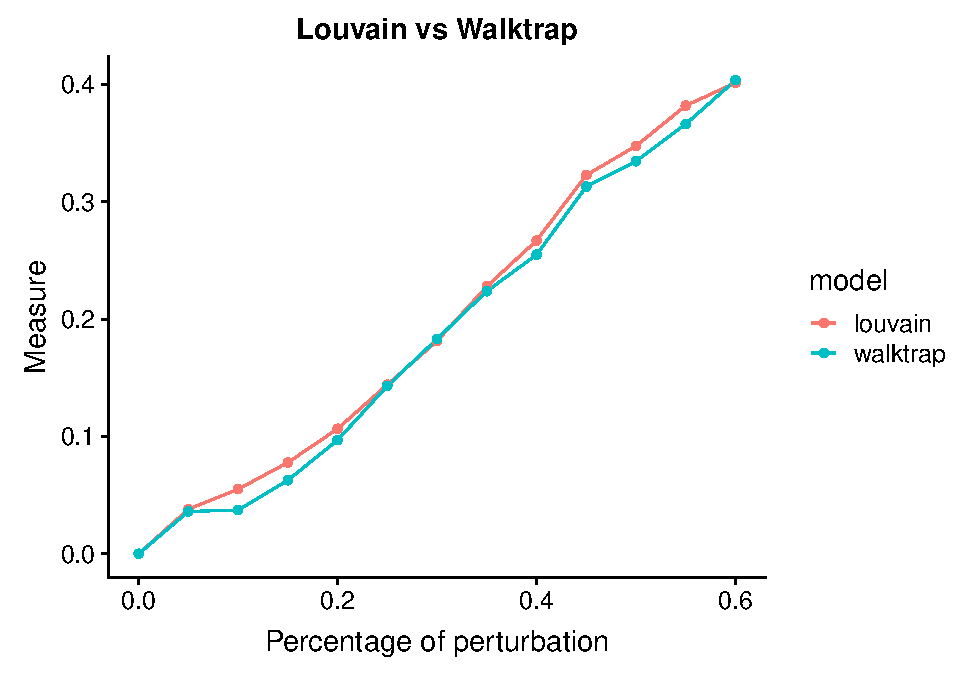
\includegraphics{Figure_Paper_files/figure-latex/unnamed-chunk-4-2.pdf}

\begin{Shaded}
\begin{Highlighting}[]
\CommentTok{#3}
\NormalTok{comp <-}\StringTok{ }\KeywordTok{robinCompare}\NormalTok{(}\DataTypeTok{graph=}\NormalTok{graph, }\DataTypeTok{method1=}\StringTok{"louvain"}\NormalTok{,}
                \DataTypeTok{method2=}\StringTok{"labelProp"}\NormalTok{, }\DataTypeTok{measure=}\StringTok{"vi"}\NormalTok{, }\DataTypeTok{type=}\StringTok{"independent"}\NormalTok{)}
\end{Highlighting}
\end{Shaded}

\begin{verbatim}
## [1] 31
## [1] 61
## [1] 92
## [1] 123
## [1] 153
## [1] 184
## [1] 215
## [1] 245
## [1] 276
## [1] 306
## [1] 337
## [1] 368
\end{verbatim}

\begin{Shaded}
\begin{Highlighting}[]
\KeywordTok{plotRobin}\NormalTok{(}\DataTypeTok{graph=}\NormalTok{graph, }\DataTypeTok{model1=}\NormalTok{comp}\OperatorTok{$}\NormalTok{Mean1, }\DataTypeTok{model2=}\NormalTok{comp}\OperatorTok{$}\NormalTok{Mean2, }\DataTypeTok{measure=}\StringTok{"vi"}\NormalTok{, }
\DataTypeTok{legend=}\KeywordTok{c}\NormalTok{(}\StringTok{"louvain"}\NormalTok{, }\StringTok{"labelProp"}\NormalTok{), }\DataTypeTok{title=}\StringTok{"Louvain vs LabelProp"}\NormalTok{)}
\end{Highlighting}
\end{Shaded}

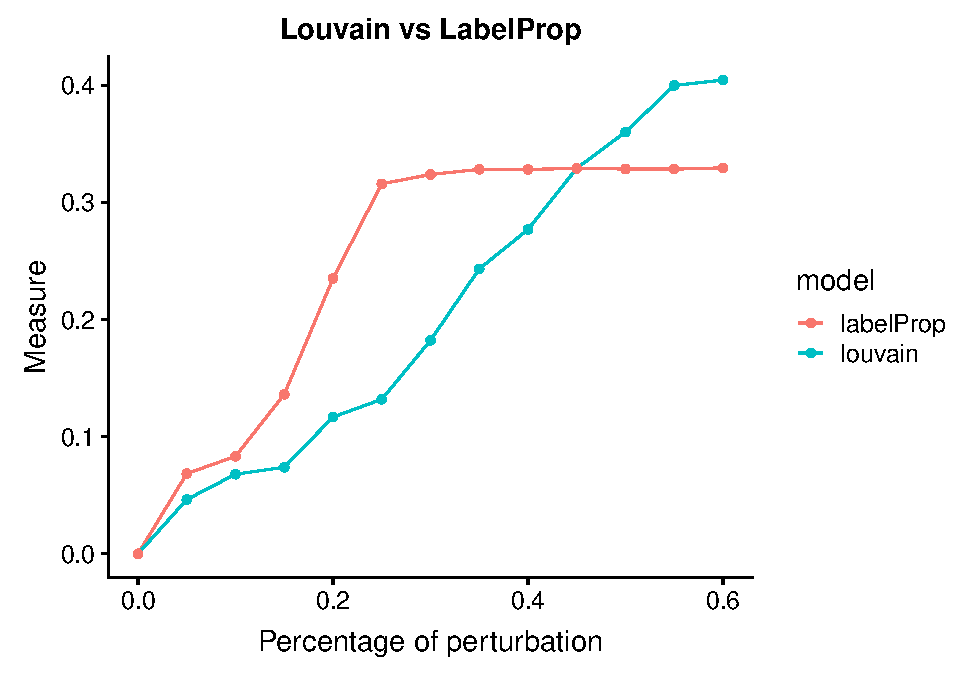
\includegraphics{Figure_Paper_files/figure-latex/unnamed-chunk-4-3.pdf}

\begin{Shaded}
\begin{Highlighting}[]
\CommentTok{#4}
\NormalTok{comp <-}\StringTok{ }\KeywordTok{robinCompare}\NormalTok{(}\DataTypeTok{graph=}\NormalTok{graph, }\DataTypeTok{method1=}\StringTok{"louvain"}\NormalTok{,}
                \DataTypeTok{method2=}\StringTok{"leadingEigen"}\NormalTok{, }\DataTypeTok{measure=}\StringTok{"vi"}\NormalTok{, }\DataTypeTok{type=}\StringTok{"independent"}\NormalTok{)}
\end{Highlighting}
\end{Shaded}

\begin{verbatim}
## [1] 31
## [1] 61
## [1] 92
## [1] 123
## [1] 153
## [1] 184
## [1] 215
## [1] 245
## [1] 276
## [1] 306
## [1] 337
## [1] 368
\end{verbatim}

\begin{Shaded}
\begin{Highlighting}[]
\KeywordTok{plotRobin}\NormalTok{(}\DataTypeTok{graph=}\NormalTok{graph, }\DataTypeTok{model1=}\NormalTok{comp}\OperatorTok{$}\NormalTok{Mean1, }\DataTypeTok{model2=}\NormalTok{comp}\OperatorTok{$}\NormalTok{Mean2, }\DataTypeTok{measure=}\StringTok{"vi"}\NormalTok{, }
\DataTypeTok{legend=}\KeywordTok{c}\NormalTok{(}\StringTok{"louvain"}\NormalTok{, }\StringTok{"leadingEigen"}\NormalTok{), }\DataTypeTok{title=}\StringTok{"Louvain vs LeadingEigen"}\NormalTok{)}
\end{Highlighting}
\end{Shaded}

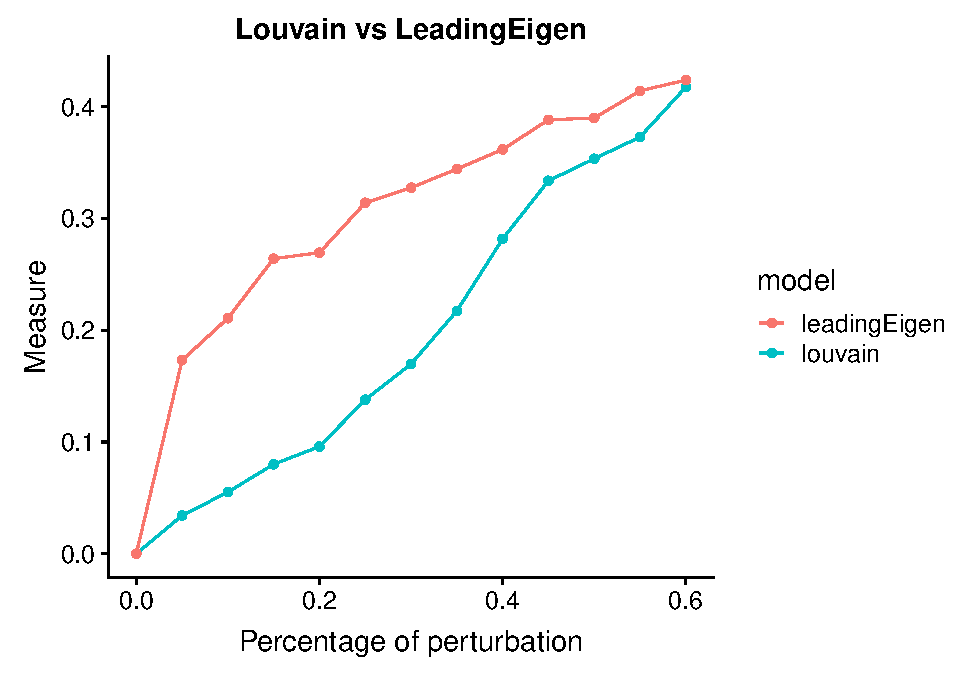
\includegraphics{Figure_Paper_files/figure-latex/unnamed-chunk-4-4.pdf}

\begin{Shaded}
\begin{Highlighting}[]
\CommentTok{#5}
\NormalTok{comp <-}\StringTok{ }\KeywordTok{robinCompare}\NormalTok{(}\DataTypeTok{graph=}\NormalTok{graph, }\DataTypeTok{method1=}\StringTok{"louvain"}\NormalTok{,}
                \DataTypeTok{method2=}\StringTok{"infomap"}\NormalTok{, }\DataTypeTok{measure=}\StringTok{"vi"}\NormalTok{, }\DataTypeTok{type=}\StringTok{"independent"}\NormalTok{)}
\end{Highlighting}
\end{Shaded}

\begin{verbatim}
## [1] 31
## [1] 61
## [1] 92
## [1] 123
## [1] 153
## [1] 184
## [1] 215
## [1] 245
## [1] 276
## [1] 306
## [1] 337
## [1] 368
\end{verbatim}

\begin{Shaded}
\begin{Highlighting}[]
\KeywordTok{plotRobin}\NormalTok{(}\DataTypeTok{graph=}\NormalTok{graph, }\DataTypeTok{model1=}\NormalTok{comp}\OperatorTok{$}\NormalTok{Mean1, }\DataTypeTok{model2=}\NormalTok{comp}\OperatorTok{$}\NormalTok{Mean2, }\DataTypeTok{measure=}\StringTok{"vi"}\NormalTok{, }
\DataTypeTok{legend=}\KeywordTok{c}\NormalTok{(}\StringTok{"louvain"}\NormalTok{, }\StringTok{"infomap"}\NormalTok{), }\DataTypeTok{title=}\StringTok{"Louvain vs Infomap"}\NormalTok{)}
\end{Highlighting}
\end{Shaded}

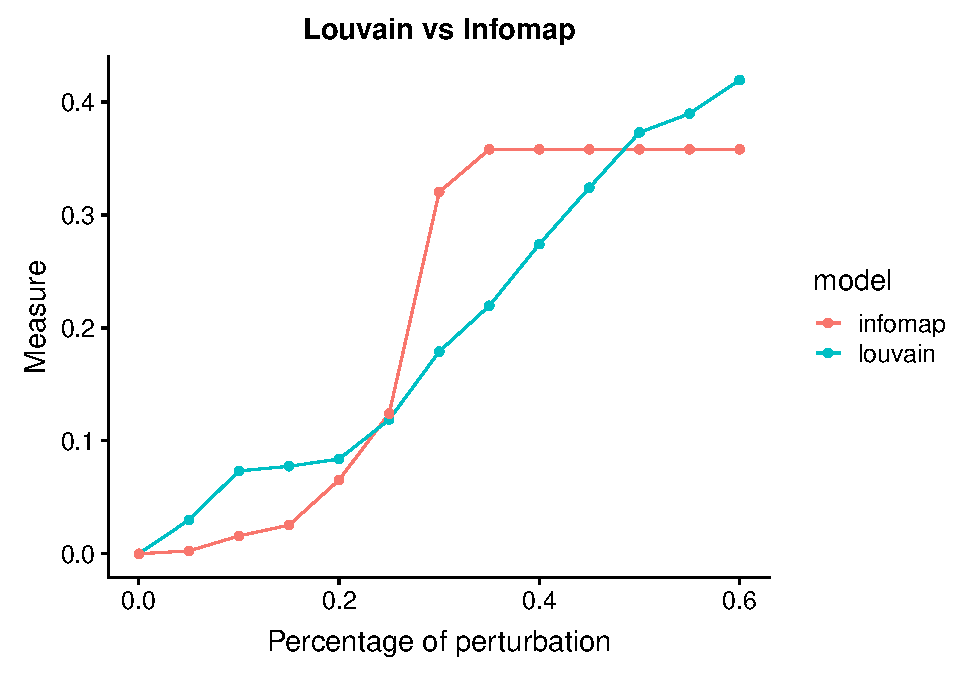
\includegraphics{Figure_Paper_files/figure-latex/unnamed-chunk-4-5.pdf}

\begin{Shaded}
\begin{Highlighting}[]
\CommentTok{#6}
\NormalTok{comp <-}\StringTok{ }\KeywordTok{robinCompare}\NormalTok{(}\DataTypeTok{graph=}\NormalTok{graph, }\DataTypeTok{method1=}\StringTok{"louvain"}\NormalTok{,}
                \DataTypeTok{method2=}\StringTok{"edgeBetweenness"}\NormalTok{, }\DataTypeTok{measure=}\StringTok{"vi"}\NormalTok{, }\DataTypeTok{type=}\StringTok{"independent"}\NormalTok{)}
\end{Highlighting}
\end{Shaded}

\begin{verbatim}
## [1] 31
## [1] 61
## [1] 92
## [1] 123
## [1] 153
## [1] 184
## [1] 215
## [1] 245
## [1] 276
## [1] 306
## [1] 337
## [1] 368
\end{verbatim}

\begin{Shaded}
\begin{Highlighting}[]
\KeywordTok{plotRobin}\NormalTok{(}\DataTypeTok{graph=}\NormalTok{graph, }\DataTypeTok{model1=}\NormalTok{comp}\OperatorTok{$}\NormalTok{Mean1, }\DataTypeTok{model2=}\NormalTok{comp}\OperatorTok{$}\NormalTok{Mean2, }\DataTypeTok{measure=}\StringTok{"vi"}\NormalTok{, }
\DataTypeTok{legend=}\KeywordTok{c}\NormalTok{(}\StringTok{"louvain"}\NormalTok{, }\StringTok{"edgeBetweenness"}\NormalTok{), }\DataTypeTok{title=}\StringTok{"Louvain vs EdgeBetweenness"}\NormalTok{)}
\end{Highlighting}
\end{Shaded}

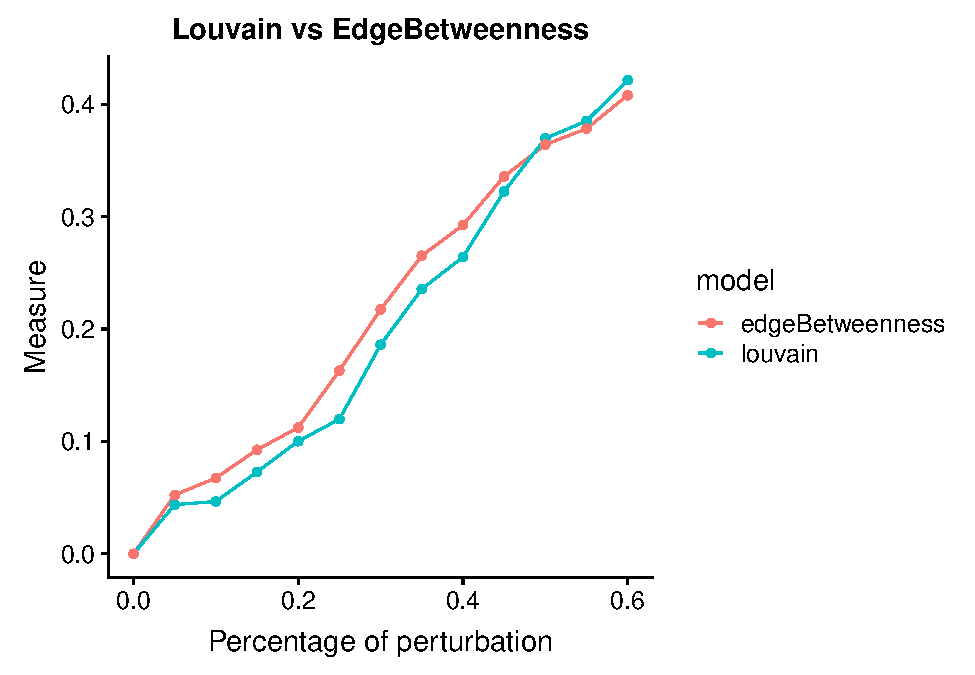
\includegraphics{Figure_Paper_files/figure-latex/unnamed-chunk-4-6.pdf}

\begin{Shaded}
\begin{Highlighting}[]
\CommentTok{#7}
\NormalTok{comp <-}\StringTok{ }\KeywordTok{robinCompare}\NormalTok{(}\DataTypeTok{graph=}\NormalTok{graph, }\DataTypeTok{method1=}\StringTok{"louvain"}\NormalTok{,}
                \DataTypeTok{method2=}\StringTok{"spinglass"}\NormalTok{, }\DataTypeTok{measure=}\StringTok{"vi"}\NormalTok{, }\DataTypeTok{type=}\StringTok{"independent"}\NormalTok{)}
\end{Highlighting}
\end{Shaded}

\begin{verbatim}
## [1] 31
## [1] 61
## [1] 92
## [1] 123
## [1] 153
## [1] 184
## [1] 215
## [1] 245
## [1] 276
## [1] 306
## [1] 337
## [1] 368
\end{verbatim}

\begin{Shaded}
\begin{Highlighting}[]
\KeywordTok{plotRobin}\NormalTok{(}\DataTypeTok{graph=}\NormalTok{graph, }\DataTypeTok{model1=}\NormalTok{comp}\OperatorTok{$}\NormalTok{Mean1, }\DataTypeTok{model2=}\NormalTok{comp}\OperatorTok{$}\NormalTok{Mean2, }\DataTypeTok{measure=}\StringTok{"vi"}\NormalTok{, }
\DataTypeTok{legend=}\KeywordTok{c}\NormalTok{(}\StringTok{"louvain"}\NormalTok{, }\StringTok{"spinglass"}\NormalTok{), }\DataTypeTok{title=}\StringTok{"Louvain vs Spinglass"}\NormalTok{)}
\end{Highlighting}
\end{Shaded}

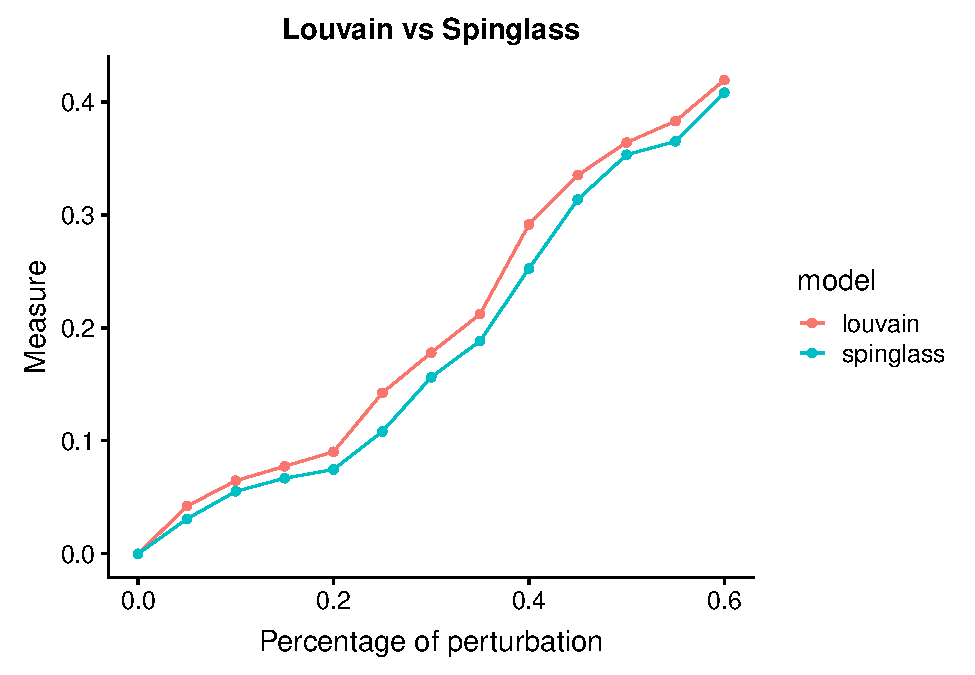
\includegraphics{Figure_Paper_files/figure-latex/unnamed-chunk-4-7.pdf}

\section{Fig.7 Different Measures with simulated data (algorithm
louvain)}\label{fig.7-different-measures-with-simulated-data-algorithm-louvain}

\begin{Shaded}
\begin{Highlighting}[]
\KeywordTok{setwd}\NormalTok{(}\StringTok{"/media/vpoli/MYFILES/CNR Tigem/Tutto per ROBIN/Dati/dati simulati"}\NormalTok{)}
\NormalTok{list.filenames<-}\KeywordTok{list.files}\NormalTok{(}\DataTypeTok{pattern=}\StringTok{".edgelist"}\NormalTok{)}
\NormalTok{BayesFactorVI<-}\OtherTok{NULL}
\NormalTok{BayesFactorNMI<-}\OtherTok{NULL}
\NormalTok{BayesFactorsplitjoin<-}\OtherTok{NULL}
\NormalTok{BayesFactoradjrand<-}\OtherTok{NULL}
\ControlFlowTok{for}\NormalTok{ (i }\ControlFlowTok{in} \DecValTok{1}\OperatorTok{:}\KeywordTok{length}\NormalTok{(list.filenames))}
\NormalTok{\{}
\NormalTok{file<-list.filenames[i]}
\NormalTok{graph<-}\KeywordTok{prepGraph}\NormalTok{(file, }\DataTypeTok{file.format =}\StringTok{"edgelist"}\NormalTok{,}\DataTypeTok{numbers =} \OtherTok{TRUE}\NormalTok{)}
\NormalTok{graph}

\NormalTok{graphRandom <-}\StringTok{ }\KeywordTok{random}\NormalTok{(graph)}
\NormalTok{graphRandom}

\CommentTok{#VI}
\NormalTok{Proc <-}\KeywordTok{robinRobust}\NormalTok{(}\DataTypeTok{graph=}\NormalTok{graph,}\DataTypeTok{graphRandom=}\NormalTok{graphRandom, }\DataTypeTok{method=}\StringTok{"louvain"}\NormalTok{,}
                       \DataTypeTok{type=}\StringTok{"independent"}\NormalTok{,}\DataTypeTok{measure =} \StringTok{"vi"}\NormalTok{)}
\NormalTok{BF<-}\KeywordTok{robinGPTest}\NormalTok{(}\DataTypeTok{ratio=}\NormalTok{Proc}\OperatorTok{$}\NormalTok{ratios)}
\NormalTok{df<-}\KeywordTok{data.frame}\NormalTok{(file,BF)}
\NormalTok{BayesFactorVI<-}\KeywordTok{rbind}\NormalTok{(BayesFactorVI,df)}


\CommentTok{#NMI}
\NormalTok{Proc <-}\KeywordTok{robinRobust}\NormalTok{(}\DataTypeTok{graph=}\NormalTok{graph,}\DataTypeTok{graphRandom=}\NormalTok{graphRandom, }\DataTypeTok{method=}\StringTok{"louvain"}\NormalTok{,}
                 \DataTypeTok{type=}\StringTok{"independent"}\NormalTok{,}\DataTypeTok{measure =} \StringTok{"nmi"}\NormalTok{)}
\NormalTok{BF<-}\KeywordTok{robinGPTest}\NormalTok{(}\DataTypeTok{ratio=}\NormalTok{Proc}\OperatorTok{$}\NormalTok{ratios)}
\NormalTok{df<-}\KeywordTok{data.frame}\NormalTok{(file,BF)}
\NormalTok{BayesFactorNMI<-}\KeywordTok{rbind}\NormalTok{(BayesFactorNMI,df)}

\CommentTok{#split-join}
\NormalTok{Proc <-}\KeywordTok{robinRobust}\NormalTok{(}\DataTypeTok{graph=}\NormalTok{graph,}\DataTypeTok{graphRandom=}\NormalTok{graphRandom, }\DataTypeTok{method=}\StringTok{"louvain"}\NormalTok{,}
                 \DataTypeTok{type=}\StringTok{"independent"}\NormalTok{,}\DataTypeTok{measure =} \StringTok{"split.join"}\NormalTok{)}
\NormalTok{BF<-}\KeywordTok{robinGPTest}\NormalTok{(}\DataTypeTok{ratio=}\NormalTok{Proc}\OperatorTok{$}\NormalTok{ratios)}
\NormalTok{df<-}\KeywordTok{data.frame}\NormalTok{(file,BF)}
\NormalTok{BayesFactorsplitjoin<-}\KeywordTok{rbind}\NormalTok{(BayesFactorsplitjoin,df)}

\CommentTok{#adj rand}
\NormalTok{Proc <-}\KeywordTok{robinRobust}\NormalTok{(}\DataTypeTok{graph=}\NormalTok{graph,}\DataTypeTok{graphRandom=}\NormalTok{graphRandom, }\DataTypeTok{method=}\StringTok{"louvain"}\NormalTok{,}
                 \DataTypeTok{type=}\StringTok{"independent"}\NormalTok{,}\DataTypeTok{measure =} \StringTok{"adjusted.rand"}\NormalTok{)}
\NormalTok{BF<-}\KeywordTok{robinGPTest}\NormalTok{(}\DataTypeTok{ratio=}\NormalTok{Proc}\OperatorTok{$}\NormalTok{ratios)}
\NormalTok{df<-}\KeywordTok{data.frame}\NormalTok{(file,BF)}
\NormalTok{BayesFactoradjrand<-}\KeywordTok{rbind}\NormalTok{(BayesFactoradjrand,df)}

\NormalTok{\}}
\end{Highlighting}
\end{Shaded}

\begin{verbatim}
## [1] 502
## [1] 1004
## [1] 1506
## [1] 2008
## [1] 2510
## [1] 3012
## [1] 3514
## [1] 4016
## [1] 4518
## [1] 5020
## [1] 5522
## [1] 6024
##  Profile  1 
##  Profile  2 
## [1] 502
## [1] 1004
## [1] 1506
## [1] 2008
## [1] 2510
## [1] 3012
## [1] 3514
## [1] 4016
## [1] 4518
## [1] 5020
## [1] 5522
## [1] 6024
##  Profile  1 
##  Profile  2 
## [1] 502
## [1] 1004
## [1] 1506
## [1] 2008
## [1] 2510
## [1] 3012
## [1] 3514
## [1] 4016
## [1] 4518
## [1] 5020
## [1] 5522
## [1] 6024
##  Profile  1 
##  Profile  2 
## [1] 502
## [1] 1004
## [1] 1506
## [1] 2008
## [1] 2510
## [1] 3012
## [1] 3514
## [1] 4016
## [1] 4518
## [1] 5020
## [1] 5522
## [1] 6024
##  Profile  1 
##  Profile  2 
## [1] 502
## [1] 1004
## [1] 1507
## [1] 2009
## [1] 2511
## [1] 3013
## [1] 3515
## [1] 4018
## [1] 4520
## [1] 5022
## [1] 5524
## [1] 6026
##  Profile  1 
##  Profile  2 
## [1] 502
## [1] 1004
## [1] 1507
## [1] 2009
## [1] 2511
## [1] 3013
## [1] 3515
## [1] 4018
## [1] 4520
## [1] 5022
## [1] 5524
## [1] 6026
##  Profile  1 
##  Profile  2 
## [1] 502
## [1] 1004
## [1] 1507
## [1] 2009
## [1] 2511
## [1] 3013
## [1] 3515
## [1] 4018
## [1] 4520
## [1] 5022
## [1] 5524
## [1] 6026
##  Profile  1 
##  Profile  2 
## [1] 502
## [1] 1004
## [1] 1507
## [1] 2009
## [1] 2511
## [1] 3013
## [1] 3515
## [1] 4018
## [1] 4520
## [1] 5022
## [1] 5524
## [1] 6026
##  Profile  1 
##  Profile  2 
## [1] 502
## [1] 1004
## [1] 1507
## [1] 2009
## [1] 2511
## [1] 3014
## [1] 3516
## [1] 4018
## [1] 4520
## [1] 5022
## [1] 5525
## [1] 6027
##  Profile  1 
##  Profile  2 
## [1] 502
## [1] 1004
## [1] 1507
## [1] 2009
## [1] 2511
## [1] 3014
## [1] 3516
## [1] 4018
## [1] 4520
## [1] 5022
## [1] 5525
## [1] 6027
##  Profile  1 
##  Profile  2 
## [1] 502
## [1] 1004
## [1] 1507
## [1] 2009
## [1] 2511
## [1] 3014
## [1] 3516
## [1] 4018
## [1] 4520
## [1] 5022
## [1] 5525
## [1] 6027
##  Profile  1 
##  Profile  2 
## [1] 502
## [1] 1004
## [1] 1507
## [1] 2009
## [1] 2511
## [1] 3014
## [1] 3516
## [1] 4018
## [1] 4520
## [1] 5022
## [1] 5525
## [1] 6027
##  Profile  1 
##  Profile  2 
## [1] 502
## [1] 1005
## [1] 1508
## [1] 2010
## [1] 2512
## [1] 3015
## [1] 3518
## [1] 4020
## [1] 4522
## [1] 5025
## [1] 5528
## [1] 6030
##  Profile  1 
##  Profile  2 
## [1] 502
## [1] 1005
## [1] 1508
## [1] 2010
## [1] 2512
## [1] 3015
## [1] 3518
## [1] 4020
## [1] 4522
## [1] 5025
## [1] 5528
## [1] 6030
##  Profile  1 
##  Profile  2 
## [1] 502
## [1] 1005
## [1] 1508
## [1] 2010
## [1] 2512
## [1] 3015
## [1] 3518
## [1] 4020
## [1] 4522
## [1] 5025
## [1] 5528
## [1] 6030
##  Profile  1 
##  Profile  2 
## [1] 502
## [1] 1005
## [1] 1508
## [1] 2010
## [1] 2512
## [1] 3015
## [1] 3518
## [1] 4020
## [1] 4522
## [1] 5025
## [1] 5528
## [1] 6030
##  Profile  1 
##  Profile  2 
## [1] 502
## [1] 1004
## [1] 1507
## [1] 2009
## [1] 2511
## [1] 3013
## [1] 3515
## [1] 4018
## [1] 4520
## [1] 5022
## [1] 5524
## [1] 6026
##  Profile  1 
##  Profile  2 
## [1] 502
## [1] 1004
## [1] 1507
## [1] 2009
## [1] 2511
## [1] 3013
## [1] 3515
## [1] 4018
## [1] 4520
## [1] 5022
## [1] 5524
## [1] 6026
##  Profile  1 
##  Profile  2 
## [1] 502
## [1] 1004
## [1] 1507
## [1] 2009
## [1] 2511
## [1] 3013
## [1] 3515
## [1] 4018
## [1] 4520
## [1] 5022
## [1] 5524
## [1] 6026
##  Profile  1 
##  Profile  2 
## [1] 502
## [1] 1004
## [1] 1507
## [1] 2009
## [1] 2511
## [1] 3013
## [1] 3515
## [1] 4018
## [1] 4520
## [1] 5022
## [1] 5524
## [1] 6026
##  Profile  1 
##  Profile  2 
## [1] 502
## [1] 1004
## [1] 1506
## [1] 2008
## [1] 2510
## [1] 3013
## [1] 3515
## [1] 4017
## [1] 4519
## [1] 5021
## [1] 5523
## [1] 6025
##  Profile  1 
##  Profile  2 
## [1] 502
## [1] 1004
## [1] 1506
## [1] 2008
## [1] 2510
## [1] 3013
## [1] 3515
## [1] 4017
## [1] 4519
## [1] 5021
## [1] 5523
## [1] 6025
##  Profile  1 
##  Profile  2 
## [1] 502
## [1] 1004
## [1] 1506
## [1] 2008
## [1] 2510
## [1] 3013
## [1] 3515
## [1] 4017
## [1] 4519
## [1] 5021
## [1] 5523
## [1] 6025
##  Profile  1 
##  Profile  2 
## [1] 502
## [1] 1004
## [1] 1506
## [1] 2008
## [1] 2510
## [1] 3013
## [1] 3515
## [1] 4017
## [1] 4519
## [1] 5021
## [1] 5523
## [1] 6025
##  Profile  1 
##  Profile  2 
## [1] 503
## [1] 1005
## [1] 1508
## [1] 2010
## [1] 2513
## [1] 3016
## [1] 3518
## [1] 4021
## [1] 4523
## [1] 5026
## [1] 5529
## [1] 6031
##  Profile  1 
##  Profile  2 
## [1] 503
## [1] 1005
## [1] 1508
## [1] 2010
## [1] 2513
## [1] 3016
## [1] 3518
## [1] 4021
## [1] 4523
## [1] 5026
## [1] 5529
## [1] 6031
##  Profile  1 
##  Profile  2 
## [1] 503
## [1] 1005
## [1] 1508
## [1] 2010
## [1] 2513
## [1] 3016
## [1] 3518
## [1] 4021
## [1] 4523
## [1] 5026
## [1] 5529
## [1] 6031
##  Profile  1 
##  Profile  2 
## [1] 503
## [1] 1005
## [1] 1508
## [1] 2010
## [1] 2513
## [1] 3016
## [1] 3518
## [1] 4021
## [1] 4523
## [1] 5026
## [1] 5529
## [1] 6031
##  Profile  1 
##  Profile  2 
## [1] 502
## [1] 1005
## [1] 1507
## [1] 2009
## [1] 2512
## [1] 3014
## [1] 3516
## [1] 4019
## [1] 4521
## [1] 5024
## [1] 5526
## [1] 6028
##  Profile  1 
##  Profile  2 
## [1] 502
## [1] 1005
## [1] 1507
## [1] 2009
## [1] 2512
## [1] 3014
## [1] 3516
## [1] 4019
## [1] 4521
## [1] 5024
## [1] 5526
## [1] 6028
##  Profile  1 
##  Profile  2 
## [1] 502
## [1] 1005
## [1] 1507
## [1] 2009
## [1] 2512
## [1] 3014
## [1] 3516
## [1] 4019
## [1] 4521
## [1] 5024
## [1] 5526
## [1] 6028
##  Profile  1 
##  Profile  2 
## [1] 502
## [1] 1005
## [1] 1507
## [1] 2009
## [1] 2512
## [1] 3014
## [1] 3516
## [1] 4019
## [1] 4521
## [1] 5024
## [1] 5526
## [1] 6028
##  Profile  1 
##  Profile  2 
## [1] 502
## [1] 1004
## [1] 1505
## [1] 2007
## [1] 2509
## [1] 3011
## [1] 3513
## [1] 4014
## [1] 4516
## [1] 5018
## [1] 5520
## [1] 6022
##  Profile  1 
##  Profile  2 
## [1] 502
## [1] 1004
## [1] 1505
## [1] 2007
## [1] 2509
## [1] 3011
## [1] 3513
## [1] 4014
## [1] 4516
## [1] 5018
## [1] 5520
## [1] 6022
##  Profile  1 
##  Profile  2 
## [1] 502
## [1] 1004
## [1] 1505
## [1] 2007
## [1] 2509
## [1] 3011
## [1] 3513
## [1] 4014
## [1] 4516
## [1] 5018
## [1] 5520
## [1] 6022
##  Profile  1 
##  Profile  2 
## [1] 502
## [1] 1004
## [1] 1505
## [1] 2007
## [1] 2509
## [1] 3011
## [1] 3513
## [1] 4014
## [1] 4516
## [1] 5018
## [1] 5520
## [1] 6022
##  Profile  1 
##  Profile  2 
## [1] 502
## [1] 1005
## [1] 1507
## [1] 2009
## [1] 2512
## [1] 3014
## [1] 3516
## [1] 4018
## [1] 4521
## [1] 5023
## [1] 5525
## [1] 6028
##  Profile  1 
##  Profile  2 
## [1] 502
## [1] 1005
## [1] 1507
## [1] 2009
## [1] 2512
## [1] 3014
## [1] 3516
## [1] 4018
## [1] 4521
## [1] 5023
## [1] 5525
## [1] 6028
##  Profile  1 
##  Profile  2 
## [1] 502
## [1] 1005
## [1] 1507
## [1] 2009
## [1] 2512
## [1] 3014
## [1] 3516
## [1] 4018
## [1] 4521
## [1] 5023
## [1] 5525
## [1] 6028
##  Profile  1 
##  Profile  2 
## [1] 502
## [1] 1005
## [1] 1507
## [1] 2009
## [1] 2512
## [1] 3014
## [1] 3516
## [1] 4018
## [1] 4521
## [1] 5023
## [1] 5525
## [1] 6028
##  Profile  1 
##  Profile  2 
## [1] 502
## [1] 1004
## [1] 1506
## [1] 2008
## [1] 2510
## [1] 3012
## [1] 3514
## [1] 4016
## [1] 4518
## [1] 5020
## [1] 5523
## [1] 6025
##  Profile  1 
##  Profile  2 
## [1] 502
## [1] 1004
## [1] 1506
## [1] 2008
## [1] 2510
## [1] 3012
## [1] 3514
## [1] 4016
## [1] 4518
## [1] 5020
## [1] 5523
## [1] 6025
##  Profile  1 
##  Profile  2 
## [1] 502
## [1] 1004
## [1] 1506
## [1] 2008
## [1] 2510
## [1] 3012
## [1] 3514
## [1] 4016
## [1] 4518
## [1] 5020
## [1] 5523
## [1] 6025
##  Profile  1 
##  Profile  2 
## [1] 502
## [1] 1004
## [1] 1506
## [1] 2008
## [1] 2510
## [1] 3012
## [1] 3514
## [1] 4016
## [1] 4518
## [1] 5020
## [1] 5523
## [1] 6025
##  Profile  1 
##  Profile  2 
## [1] 502
## [1] 1004
## [1] 1505
## [1] 2007
## [1] 2509
## [1] 3011
## [1] 3513
## [1] 4014
## [1] 4516
## [1] 5018
## [1] 5520
## [1] 6022
##  Profile  1 
##  Profile  2 
## [1] 502
## [1] 1004
## [1] 1505
## [1] 2007
## [1] 2509
## [1] 3011
## [1] 3513
## [1] 4014
## [1] 4516
## [1] 5018
## [1] 5520
## [1] 6022
##  Profile  1 
##  Profile  2 
## [1] 502
## [1] 1004
## [1] 1505
## [1] 2007
## [1] 2509
## [1] 3011
## [1] 3513
## [1] 4014
## [1] 4516
## [1] 5018
## [1] 5520
## [1] 6022
##  Profile  1 
##  Profile  2 
## [1] 502
## [1] 1004
## [1] 1505
## [1] 2007
## [1] 2509
## [1] 3011
## [1] 3513
## [1] 4014
## [1] 4516
## [1] 5018
## [1] 5520
## [1] 6022
##  Profile  1 
##  Profile  2 
## [1] 502
## [1] 1004
## [1] 1506
## [1] 2008
## [1] 2510
## [1] 3013
## [1] 3515
## [1] 4017
## [1] 4519
## [1] 5021
## [1] 5523
## [1] 6025
##  Profile  1 
##  Profile  2 
## [1] 502
## [1] 1004
## [1] 1506
## [1] 2008
## [1] 2510
## [1] 3013
## [1] 3515
## [1] 4017
## [1] 4519
## [1] 5021
## [1] 5523
## [1] 6025
##  Profile  1 
##  Profile  2 
## [1] 502
## [1] 1004
## [1] 1506
## [1] 2008
## [1] 2510
## [1] 3013
## [1] 3515
## [1] 4017
## [1] 4519
## [1] 5021
## [1] 5523
## [1] 6025
##  Profile  1 
##  Profile  2 
## [1] 502
## [1] 1004
## [1] 1506
## [1] 2008
## [1] 2510
## [1] 3013
## [1] 3515
## [1] 4017
## [1] 4519
## [1] 5021
## [1] 5523
## [1] 6025
##  Profile  1 
##  Profile  2 
## [1] 502
## [1] 1004
## [1] 1506
## [1] 2008
## [1] 2510
## [1] 3012
## [1] 3514
## [1] 4016
## [1] 4518
## [1] 5020
## [1] 5521
## [1] 6023
##  Profile  1 
##  Profile  2 
## [1] 502
## [1] 1004
## [1] 1506
## [1] 2008
## [1] 2510
## [1] 3012
## [1] 3514
## [1] 4016
## [1] 4518
## [1] 5020
## [1] 5521
## [1] 6023
##  Profile  1 
##  Profile  2 
## [1] 502
## [1] 1004
## [1] 1506
## [1] 2008
## [1] 2510
## [1] 3012
## [1] 3514
## [1] 4016
## [1] 4518
## [1] 5020
## [1] 5521
## [1] 6023
##  Profile  1 
##  Profile  2 
## [1] 502
## [1] 1004
## [1] 1506
## [1] 2008
## [1] 2510
## [1] 3012
## [1] 3514
## [1] 4016
## [1] 4518
## [1] 5020
## [1] 5521
## [1] 6023
##  Profile  1 
##  Profile  2 
## [1] 502
## [1] 1005
## [1] 1507
## [1] 2010
## [1] 2512
## [1] 3015
## [1] 3517
## [1] 4020
## [1] 4522
## [1] 5024
## [1] 5527
## [1] 6029
##  Profile  1 
##  Profile  2 
## [1] 502
## [1] 1005
## [1] 1507
## [1] 2010
## [1] 2512
## [1] 3015
## [1] 3517
## [1] 4020
## [1] 4522
## [1] 5024
## [1] 5527
## [1] 6029
##  Profile  1 
##  Profile  2 
## [1] 502
## [1] 1005
## [1] 1507
## [1] 2010
## [1] 2512
## [1] 3015
## [1] 3517
## [1] 4020
## [1] 4522
## [1] 5024
## [1] 5527
## [1] 6029
##  Profile  1 
##  Profile  2 
## [1] 502
## [1] 1005
## [1] 1507
## [1] 2010
## [1] 2512
## [1] 3015
## [1] 3517
## [1] 4020
## [1] 4522
## [1] 5024
## [1] 5527
## [1] 6029
##  Profile  1 
##  Profile  2 
## [1] 502
## [1] 1005
## [1] 1507
## [1] 2010
## [1] 2512
## [1] 3015
## [1] 3517
## [1] 4020
## [1] 4522
## [1] 5024
## [1] 5527
## [1] 6029
##  Profile  1 
##  Profile  2 
## [1] 502
## [1] 1005
## [1] 1507
## [1] 2010
## [1] 2512
## [1] 3015
## [1] 3517
## [1] 4020
## [1] 4522
## [1] 5024
## [1] 5527
## [1] 6029
##  Profile  1 
##  Profile  2 
## [1] 502
## [1] 1005
## [1] 1507
## [1] 2010
## [1] 2512
## [1] 3015
## [1] 3517
## [1] 4020
## [1] 4522
## [1] 5024
## [1] 5527
## [1] 6029
##  Profile  1 
##  Profile  2 
## [1] 502
## [1] 1005
## [1] 1507
## [1] 2010
## [1] 2512
## [1] 3015
## [1] 3517
## [1] 4020
## [1] 4522
## [1] 5024
## [1] 5527
## [1] 6029
##  Profile  1 
##  Profile  2 
## [1] 502
## [1] 1005
## [1] 1507
## [1] 2010
## [1] 2512
## [1] 3014
## [1] 3517
## [1] 4019
## [1] 4522
## [1] 5024
## [1] 5526
## [1] 6029
##  Profile  1 
##  Profile  2 
## [1] 502
## [1] 1005
## [1] 1507
## [1] 2010
## [1] 2512
## [1] 3014
## [1] 3517
## [1] 4019
## [1] 4522
## [1] 5024
## [1] 5526
## [1] 6029
##  Profile  1 
##  Profile  2 
## [1] 502
## [1] 1005
## [1] 1507
## [1] 2010
## [1] 2512
## [1] 3014
## [1] 3517
## [1] 4019
## [1] 4522
## [1] 5024
## [1] 5526
## [1] 6029
##  Profile  1 
##  Profile  2 
## [1] 502
## [1] 1005
## [1] 1507
## [1] 2010
## [1] 2512
## [1] 3014
## [1] 3517
## [1] 4019
## [1] 4522
## [1] 5024
## [1] 5526
## [1] 6029
##  Profile  1 
##  Profile  2 
## [1] 502
## [1] 1004
## [1] 1506
## [1] 2008
## [1] 2510
## [1] 3012
## [1] 3514
## [1] 4016
## [1] 4518
## [1] 5020
## [1] 5521
## [1] 6023
##  Profile  1 
##  Profile  2 
## [1] 502
## [1] 1004
## [1] 1506
## [1] 2008
## [1] 2510
## [1] 3012
## [1] 3514
## [1] 4016
## [1] 4518
## [1] 5020
## [1] 5521
## [1] 6023
##  Profile  1 
##  Profile  2 
## [1] 502
## [1] 1004
## [1] 1506
## [1] 2008
## [1] 2510
## [1] 3012
## [1] 3514
## [1] 4016
## [1] 4518
## [1] 5020
## [1] 5521
## [1] 6023
##  Profile  1 
##  Profile  2 
## [1] 502
## [1] 1004
## [1] 1506
## [1] 2008
## [1] 2510
## [1] 3012
## [1] 3514
## [1] 4016
## [1] 4518
## [1] 5020
## [1] 5521
## [1] 6023
##  Profile  1 
##  Profile  2 
## [1] 502
## [1] 1004
## [1] 1506
## [1] 2009
## [1] 2511
## [1] 3013
## [1] 3515
## [1] 4017
## [1] 4519
## [1] 5022
## [1] 5524
## [1] 6026
##  Profile  1 
##  Profile  2 
## [1] 502
## [1] 1004
## [1] 1506
## [1] 2009
## [1] 2511
## [1] 3013
## [1] 3515
## [1] 4017
## [1] 4519
## [1] 5022
## [1] 5524
## [1] 6026
##  Profile  1 
##  Profile  2 
## [1] 502
## [1] 1004
## [1] 1506
## [1] 2009
## [1] 2511
## [1] 3013
## [1] 3515
## [1] 4017
## [1] 4519
## [1] 5022
## [1] 5524
## [1] 6026
##  Profile  1 
##  Profile  2 
## [1] 502
## [1] 1004
## [1] 1506
## [1] 2009
## [1] 2511
## [1] 3013
## [1] 3515
## [1] 4017
## [1] 4519
## [1] 5022
## [1] 5524
## [1] 6026
##  Profile  1 
##  Profile  2 
## [1] 502
## [1] 1005
## [1] 1507
## [1] 2010
## [1] 2512
## [1] 3014
## [1] 3517
## [1] 4019
## [1] 4522
## [1] 5024
## [1] 5526
## [1] 6029
##  Profile  1 
##  Profile  2 
## [1] 502
## [1] 1005
## [1] 1507
## [1] 2010
## [1] 2512
## [1] 3014
## [1] 3517
## [1] 4019
## [1] 4522
## [1] 5024
## [1] 5526
## [1] 6029
##  Profile  1 
##  Profile  2 
## [1] 502
## [1] 1005
## [1] 1507
## [1] 2010
## [1] 2512
## [1] 3014
## [1] 3517
## [1] 4019
## [1] 4522
## [1] 5024
## [1] 5526
## [1] 6029
##  Profile  1 
##  Profile  2 
## [1] 502
## [1] 1005
## [1] 1507
## [1] 2010
## [1] 2512
## [1] 3014
## [1] 3517
## [1] 4019
## [1] 4522
## [1] 5024
## [1] 5526
## [1] 6029
##  Profile  1 
##  Profile  2 
## [1] 502
## [1] 1004
## [1] 1506
## [1] 2008
## [1] 2510
## [1] 3012
## [1] 3514
## [1] 4016
## [1] 4518
## [1] 5020
## [1] 5523
## [1] 6025
##  Profile  1 
##  Profile  2 
## [1] 502
## [1] 1004
## [1] 1506
## [1] 2008
## [1] 2510
## [1] 3012
## [1] 3514
## [1] 4016
## [1] 4518
## [1] 5020
## [1] 5523
## [1] 6025
##  Profile  1 
##  Profile  2 
## [1] 502
## [1] 1004
## [1] 1506
## [1] 2008
## [1] 2510
## [1] 3012
## [1] 3514
## [1] 4016
## [1] 4518
## [1] 5020
## [1] 5523
## [1] 6025
##  Profile  1 
##  Profile  2 
## [1] 502
## [1] 1004
## [1] 1506
## [1] 2008
## [1] 2510
## [1] 3012
## [1] 3514
## [1] 4016
## [1] 4518
## [1] 5020
## [1] 5523
## [1] 6025
##  Profile  1 
##  Profile  2 
## [1] 502
## [1] 1004
## [1] 1506
## [1] 2008
## [1] 2510
## [1] 3011
## [1] 3513
## [1] 4015
## [1] 4517
## [1] 5019
## [1] 5521
## [1] 6023
##  Profile  1 
##  Profile  2 
## [1] 502
## [1] 1004
## [1] 1506
## [1] 2008
## [1] 2510
## [1] 3011
## [1] 3513
## [1] 4015
## [1] 4517
## [1] 5019
## [1] 5521
## [1] 6023
##  Profile  1 
##  Profile  2 
## [1] 502
## [1] 1004
## [1] 1506
## [1] 2008
## [1] 2510
## [1] 3011
## [1] 3513
## [1] 4015
## [1] 4517
## [1] 5019
## [1] 5521
## [1] 6023
##  Profile  1 
##  Profile  2 
## [1] 502
## [1] 1004
## [1] 1506
## [1] 2008
## [1] 2510
## [1] 3011
## [1] 3513
## [1] 4015
## [1] 4517
## [1] 5019
## [1] 5521
## [1] 6023
##  Profile  1 
##  Profile  2 
## [1] 502
## [1] 1004
## [1] 1506
## [1] 2009
## [1] 2511
## [1] 3013
## [1] 3515
## [1] 4017
## [1] 4519
## [1] 5022
## [1] 5524
## [1] 6026
##  Profile  1 
##  Profile  2 
## [1] 502
## [1] 1004
## [1] 1506
## [1] 2009
## [1] 2511
## [1] 3013
## [1] 3515
## [1] 4017
## [1] 4519
## [1] 5022
## [1] 5524
## [1] 6026
##  Profile  1 
##  Profile  2 
## [1] 502
## [1] 1004
## [1] 1506
## [1] 2009
## [1] 2511
## [1] 3013
## [1] 3515
## [1] 4017
## [1] 4519
## [1] 5022
## [1] 5524
## [1] 6026
##  Profile  1 
##  Profile  2 
## [1] 502
## [1] 1004
## [1] 1506
## [1] 2009
## [1] 2511
## [1] 3013
## [1] 3515
## [1] 4017
## [1] 4519
## [1] 5022
## [1] 5524
## [1] 6026
##  Profile  1 
##  Profile  2 
## [1] 502
## [1] 1004
## [1] 1506
## [1] 2007
## [1] 2509
## [1] 3011
## [1] 3513
## [1] 4015
## [1] 4517
## [1] 5018
## [1] 5520
## [1] 6022
##  Profile  1 
##  Profile  2 
## [1] 502
## [1] 1004
## [1] 1506
## [1] 2007
## [1] 2509
## [1] 3011
## [1] 3513
## [1] 4015
## [1] 4517
## [1] 5018
## [1] 5520
## [1] 6022
##  Profile  1 
##  Profile  2 
## [1] 502
## [1] 1004
## [1] 1506
## [1] 2007
## [1] 2509
## [1] 3011
## [1] 3513
## [1] 4015
## [1] 4517
## [1] 5018
## [1] 5520
## [1] 6022
##  Profile  1 
##  Profile  2 
## [1] 502
## [1] 1004
## [1] 1506
## [1] 2007
## [1] 2509
## [1] 3011
## [1] 3513
## [1] 4015
## [1] 4517
## [1] 5018
## [1] 5520
## [1] 6022
##  Profile  1 
##  Profile  2 
## [1] 502
## [1] 1003
## [1] 1504
## [1] 2006
## [1] 2508
## [1] 3009
## [1] 3510
## [1] 4012
## [1] 4514
## [1] 5015
## [1] 5516
## [1] 6018
##  Profile  1 
##  Profile  2 
## [1] 502
## [1] 1003
## [1] 1504
## [1] 2006
## [1] 2508
## [1] 3009
## [1] 3510
## [1] 4012
## [1] 4514
## [1] 5015
## [1] 5516
## [1] 6018
##  Profile  1 
##  Profile  2 
## [1] 502
## [1] 1003
## [1] 1504
## [1] 2006
## [1] 2508
## [1] 3009
## [1] 3510
## [1] 4012
## [1] 4514
## [1] 5015
## [1] 5516
## [1] 6018
##  Profile  1 
##  Profile  2 
## [1] 502
## [1] 1003
## [1] 1504
## [1] 2006
## [1] 2508
## [1] 3009
## [1] 3510
## [1] 4012
## [1] 4514
## [1] 5015
## [1] 5516
## [1] 6018
##  Profile  1 
##  Profile  2 
## [1] 502
## [1] 1004
## [1] 1505
## [1] 2007
## [1] 2509
## [1] 3011
## [1] 3513
## [1] 4014
## [1] 4516
## [1] 5018
## [1] 5520
## [1] 6022
##  Profile  1 
##  Profile  2 
## [1] 502
## [1] 1004
## [1] 1505
## [1] 2007
## [1] 2509
## [1] 3011
## [1] 3513
## [1] 4014
## [1] 4516
## [1] 5018
## [1] 5520
## [1] 6022
##  Profile  1 
##  Profile  2 
## [1] 502
## [1] 1004
## [1] 1505
## [1] 2007
## [1] 2509
## [1] 3011
## [1] 3513
## [1] 4014
## [1] 4516
## [1] 5018
## [1] 5520
## [1] 6022
##  Profile  1 
##  Profile  2 
## [1] 502
## [1] 1004
## [1] 1505
## [1] 2007
## [1] 2509
## [1] 3011
## [1] 3513
## [1] 4014
## [1] 4516
## [1] 5018
## [1] 5520
## [1] 6022
##  Profile  1 
##  Profile  2 
## [1] 502
## [1] 1004
## [1] 1506
## [1] 2008
## [1] 2510
## [1] 3013
## [1] 3515
## [1] 4017
## [1] 4519
## [1] 5021
## [1] 5523
## [1] 6025
##  Profile  1 
##  Profile  2 
## [1] 502
## [1] 1004
## [1] 1506
## [1] 2008
## [1] 2510
## [1] 3013
## [1] 3515
## [1] 4017
## [1] 4519
## [1] 5021
## [1] 5523
## [1] 6025
##  Profile  1 
##  Profile  2 
## [1] 502
## [1] 1004
## [1] 1506
## [1] 2008
## [1] 2510
## [1] 3013
## [1] 3515
## [1] 4017
## [1] 4519
## [1] 5021
## [1] 5523
## [1] 6025
##  Profile  1 
##  Profile  2 
## [1] 502
## [1] 1004
## [1] 1506
## [1] 2008
## [1] 2510
## [1] 3013
## [1] 3515
## [1] 4017
## [1] 4519
## [1] 5021
## [1] 5523
## [1] 6025
##  Profile  1 
##  Profile  2 
## [1] 502
## [1] 1004
## [1] 1506
## [1] 2008
## [1] 2510
## [1] 3012
## [1] 3514
## [1] 4016
## [1] 4518
## [1] 5020
## [1] 5523
## [1] 6025
##  Profile  1 
##  Profile  2 
## [1] 502
## [1] 1004
## [1] 1506
## [1] 2008
## [1] 2510
## [1] 3012
## [1] 3514
## [1] 4016
## [1] 4518
## [1] 5020
## [1] 5523
## [1] 6025
##  Profile  1 
##  Profile  2 
## [1] 502
## [1] 1004
## [1] 1506
## [1] 2008
## [1] 2510
## [1] 3012
## [1] 3514
## [1] 4016
## [1] 4518
## [1] 5020
## [1] 5523
## [1] 6025
##  Profile  1 
##  Profile  2 
## [1] 502
## [1] 1004
## [1] 1506
## [1] 2008
## [1] 2510
## [1] 3012
## [1] 3514
## [1] 4016
## [1] 4518
## [1] 5020
## [1] 5523
## [1] 6025
##  Profile  1 
##  Profile  2 
## [1] 502
## [1] 1004
## [1] 1506
## [1] 2008
## [1] 2510
## [1] 3012
## [1] 3514
## [1] 4016
## [1] 4518
## [1] 5020
## [1] 5521
## [1] 6023
##  Profile  1 
##  Profile  2 
## [1] 502
## [1] 1004
## [1] 1506
## [1] 2008
## [1] 2510
## [1] 3012
## [1] 3514
## [1] 4016
## [1] 4518
## [1] 5020
## [1] 5521
## [1] 6023
##  Profile  1 
##  Profile  2 
## [1] 502
## [1] 1004
## [1] 1506
## [1] 2008
## [1] 2510
## [1] 3012
## [1] 3514
## [1] 4016
## [1] 4518
## [1] 5020
## [1] 5521
## [1] 6023
##  Profile  1 
##  Profile  2 
## [1] 502
## [1] 1004
## [1] 1506
## [1] 2008
## [1] 2510
## [1] 3012
## [1] 3514
## [1] 4016
## [1] 4518
## [1] 5020
## [1] 5521
## [1] 6023
##  Profile  1 
##  Profile  2 
## [1] 502
## [1] 1004
## [1] 1507
## [1] 2009
## [1] 2511
## [1] 3014
## [1] 3516
## [1] 4018
## [1] 4520
## [1] 5022
## [1] 5525
## [1] 6027
##  Profile  1 
##  Profile  2 
## [1] 502
## [1] 1004
## [1] 1507
## [1] 2009
## [1] 2511
## [1] 3014
## [1] 3516
## [1] 4018
## [1] 4520
## [1] 5022
## [1] 5525
## [1] 6027
##  Profile  1 
##  Profile  2 
## [1] 502
## [1] 1004
## [1] 1507
## [1] 2009
## [1] 2511
## [1] 3014
## [1] 3516
## [1] 4018
## [1] 4520
## [1] 5022
## [1] 5525
## [1] 6027
##  Profile  1 
##  Profile  2 
## [1] 502
## [1] 1004
## [1] 1507
## [1] 2009
## [1] 2511
## [1] 3014
## [1] 3516
## [1] 4018
## [1] 4520
## [1] 5022
## [1] 5525
## [1] 6027
##  Profile  1 
##  Profile  2 
## [1] 502
## [1] 1004
## [1] 1506
## [1] 2009
## [1] 2511
## [1] 3013
## [1] 3515
## [1] 4017
## [1] 4519
## [1] 5022
## [1] 5524
## [1] 6026
##  Profile  1 
##  Profile  2 
## [1] 502
## [1] 1004
## [1] 1506
## [1] 2009
## [1] 2511
## [1] 3013
## [1] 3515
## [1] 4017
## [1] 4519
## [1] 5022
## [1] 5524
## [1] 6026
##  Profile  1 
##  Profile  2 
## [1] 502
## [1] 1004
## [1] 1506
## [1] 2009
## [1] 2511
## [1] 3013
## [1] 3515
## [1] 4017
## [1] 4519
## [1] 5022
## [1] 5524
## [1] 6026
##  Profile  1 
##  Profile  2 
## [1] 502
## [1] 1004
## [1] 1506
## [1] 2009
## [1] 2511
## [1] 3013
## [1] 3515
## [1] 4017
## [1] 4519
## [1] 5022
## [1] 5524
## [1] 6026
##  Profile  1 
##  Profile  2 
## [1] 502
## [1] 1003
## [1] 1505
## [1] 2007
## [1] 2508
## [1] 3010
## [1] 3512
## [1] 4013
## [1] 4515
## [1] 5016
## [1] 5518
## [1] 6020
##  Profile  1 
##  Profile  2 
## [1] 502
## [1] 1003
## [1] 1505
## [1] 2007
## [1] 2508
## [1] 3010
## [1] 3512
## [1] 4013
## [1] 4515
## [1] 5016
## [1] 5518
## [1] 6020
##  Profile  1 
##  Profile  2 
## [1] 502
## [1] 1003
## [1] 1505
## [1] 2007
## [1] 2508
## [1] 3010
## [1] 3512
## [1] 4013
## [1] 4515
## [1] 5016
## [1] 5518
## [1] 6020
##  Profile  1 
##  Profile  2 
## [1] 502
## [1] 1003
## [1] 1505
## [1] 2007
## [1] 2508
## [1] 3010
## [1] 3512
## [1] 4013
## [1] 4515
## [1] 5016
## [1] 5518
## [1] 6020
##  Profile  1 
##  Profile  2 
## [1] 502
## [1] 1004
## [1] 1505
## [1] 2007
## [1] 2509
## [1] 3010
## [1] 3512
## [1] 4014
## [1] 4516
## [1] 5018
## [1] 5519
## [1] 6021
##  Profile  1 
##  Profile  2 
## [1] 502
## [1] 1004
## [1] 1505
## [1] 2007
## [1] 2509
## [1] 3010
## [1] 3512
## [1] 4014
## [1] 4516
## [1] 5018
## [1] 5519
## [1] 6021
##  Profile  1 
##  Profile  2 
## [1] 502
## [1] 1004
## [1] 1505
## [1] 2007
## [1] 2509
## [1] 3010
## [1] 3512
## [1] 4014
## [1] 4516
## [1] 5018
## [1] 5519
## [1] 6021
##  Profile  1 
##  Profile  2 
## [1] 502
## [1] 1004
## [1] 1505
## [1] 2007
## [1] 2509
## [1] 3010
## [1] 3512
## [1] 4014
## [1] 4516
## [1] 5018
## [1] 5519
## [1] 6021
##  Profile  1 
##  Profile  2
\end{verbatim}

\begin{Shaded}
\begin{Highlighting}[]
\KeywordTok{write.csv}\NormalTok{(BayesFactorVI,}\DataTypeTok{file=}\StringTok{"BayesFactorVSModularityVI.csv"}\NormalTok{)}
\KeywordTok{write.csv}\NormalTok{(BayesFactorNMI,}\DataTypeTok{file=}\StringTok{"BayesFactorVSModularityNMI.csv"}\NormalTok{)}
\KeywordTok{write.csv}\NormalTok{(BayesFactoradjrand,}\DataTypeTok{file=}\StringTok{"BayesFactorVSModularityadjrand.csv"}\NormalTok{)}
\KeywordTok{write.csv}\NormalTok{(BayesFactorsplitjoin,}\DataTypeTok{file=}\StringTok{"BayesFactorVSModularitysplitjoin.csv"}\NormalTok{)}


\NormalTok{####VI}
\NormalTok{BayesFactorVSModularity <-}\StringTok{ }\KeywordTok{read.csv}\NormalTok{(}\StringTok{"BayesFactorVSModularityVI.csv"}\NormalTok{)}
\KeywordTok{head}\NormalTok{(BayesFactorVSModularity)}
\end{Highlighting}
\end{Shaded}

\begin{verbatim}
##   X           file        BF
## 1 1    Q0.edgelist 33.370333
## 2 2 Q0025.edgelist  8.333360
## 3 3  Q005.edgelist  5.868360
## 4 4 Q0075.edgelist  1.843076
## 5 5   Q01.edgelist  6.275108
## 6 6 Q0125.edgelist 13.841894
\end{verbatim}

\begin{Shaded}
\begin{Highlighting}[]
\NormalTok{x<-}\KeywordTok{seq}\NormalTok{(}\DecValTok{0}\NormalTok{,}\FloatTok{0.8}\NormalTok{,}\FloatTok{0.025}\NormalTok{)}
\NormalTok{df<-}\KeywordTok{data.frame}\NormalTok{(BayesFactorVSModularity}\OperatorTok{$}\NormalTok{BF,x)}
\KeywordTok{ggplot}\NormalTok{(}\DataTypeTok{data=}\NormalTok{df, }\KeywordTok{aes}\NormalTok{(}\DataTypeTok{x=}\NormalTok{x, }\DataTypeTok{y=}\NormalTok{BayesFactorVSModularity}\OperatorTok{$}\NormalTok{BF, }\DataTypeTok{group=}\DecValTok{1}\NormalTok{)) }\OperatorTok{+}
\StringTok{    }\KeywordTok{geom_line}\NormalTok{(}\DataTypeTok{color=}\StringTok{"dark blue"}\NormalTok{)}\OperatorTok{+}
\StringTok{    }\KeywordTok{geom_point}\NormalTok{(}\DataTypeTok{color=}\StringTok{"dark blue"}\NormalTok{)}\OperatorTok{+}
\StringTok{    }\KeywordTok{xlab}\NormalTok{(}\StringTok{"Modularity"}\NormalTok{) }\OperatorTok{+}
\StringTok{    }\KeywordTok{ylab}\NormalTok{(}\StringTok{"BayesFactor"}\NormalTok{) }\OperatorTok{+}
\StringTok{    }\KeywordTok{ggtitle}\NormalTok{(}\StringTok{"VI"}\NormalTok{)}
\end{Highlighting}
\end{Shaded}

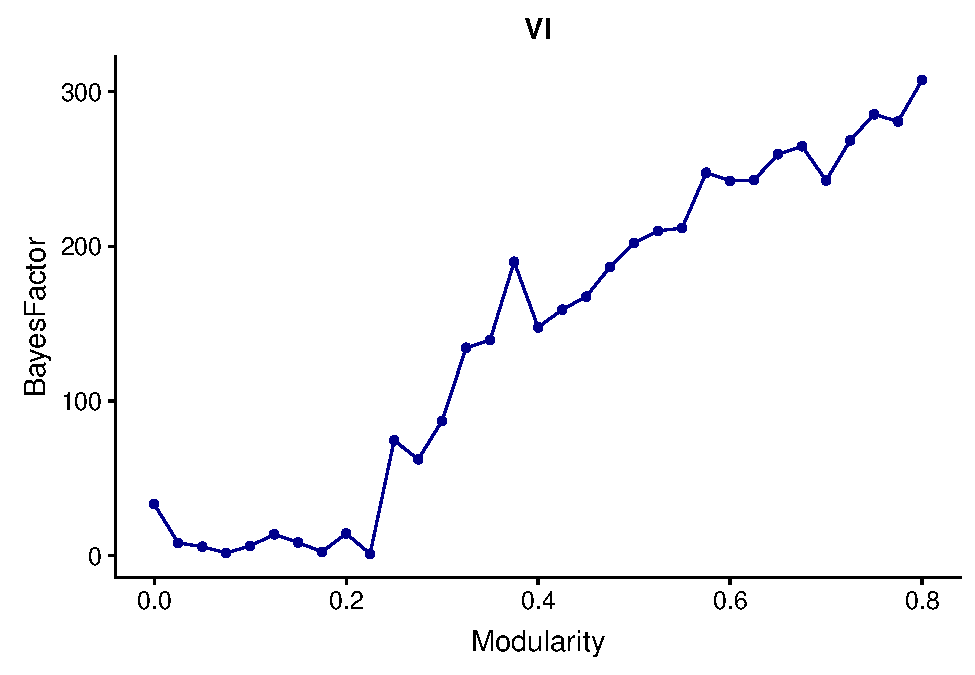
\includegraphics{Figure_Paper_files/figure-latex/unnamed-chunk-5-1.pdf}

\begin{Shaded}
\begin{Highlighting}[]
\NormalTok{###NMI}
\NormalTok{BayesFactorVSModularityNMI <-}\StringTok{ }\KeywordTok{read.csv}\NormalTok{(}\StringTok{"BayesFactorVSModularityNMI.csv"}\NormalTok{)}
\NormalTok{df<-}\KeywordTok{data.frame}\NormalTok{(BayesFactorVSModularityNMI}\OperatorTok{$}\NormalTok{BF,x)}

\KeywordTok{ggplot}\NormalTok{(}\DataTypeTok{data=}\NormalTok{df, }\KeywordTok{aes}\NormalTok{(}\DataTypeTok{x=}\NormalTok{x, }\DataTypeTok{y=}\NormalTok{BayesFactorVSModularityNMI}\OperatorTok{$}\NormalTok{BF, }\DataTypeTok{group=}\DecValTok{1}\NormalTok{)) }\OperatorTok{+}
\StringTok{    }\KeywordTok{geom_line}\NormalTok{(}\DataTypeTok{color=}\StringTok{"dark blue"}\NormalTok{)}\OperatorTok{+}
\StringTok{    }\KeywordTok{geom_point}\NormalTok{(}\DataTypeTok{color=}\StringTok{"dark blue"}\NormalTok{)}\OperatorTok{+}
\StringTok{     }\KeywordTok{xlab}\NormalTok{(}\StringTok{"Modularity"}\NormalTok{) }\OperatorTok{+}
\StringTok{    }\KeywordTok{ylab}\NormalTok{(}\StringTok{"BayesFactor"}\NormalTok{) }\OperatorTok{+}
\StringTok{    }\KeywordTok{ggtitle}\NormalTok{(}\StringTok{"NMI"}\NormalTok{)}
\end{Highlighting}
\end{Shaded}

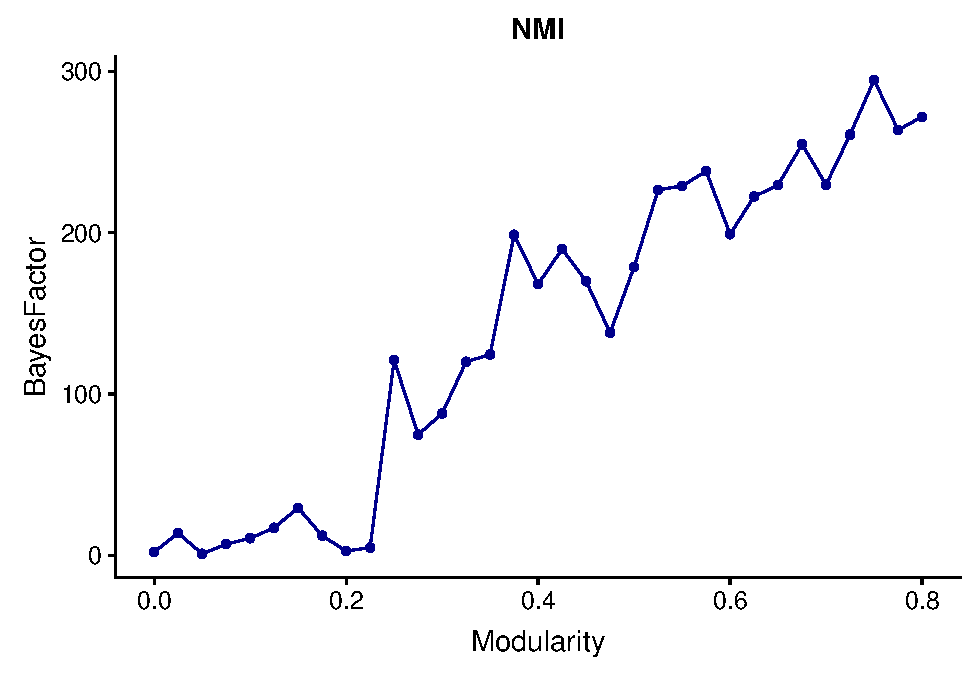
\includegraphics{Figure_Paper_files/figure-latex/unnamed-chunk-5-2.pdf}

\begin{Shaded}
\begin{Highlighting}[]
\NormalTok{###Adj rand }
\NormalTok{BayesFactorVSModularityadjrand <-}\StringTok{ }\KeywordTok{read.csv}\NormalTok{(}\StringTok{"BayesFactorVSModularityadjrand.csv"}\NormalTok{)}

\NormalTok{df<-}\KeywordTok{data.frame}\NormalTok{(BayesFactorVSModularityadjrand}\OperatorTok{$}\NormalTok{BF,x)}
\KeywordTok{ggplot}\NormalTok{(}\DataTypeTok{data=}\NormalTok{df, }\KeywordTok{aes}\NormalTok{(}\DataTypeTok{x=}\NormalTok{x, }\DataTypeTok{y=}\NormalTok{BayesFactorVSModularityadjrand}\OperatorTok{$}\NormalTok{BF, }\DataTypeTok{group=}\DecValTok{1}\NormalTok{)) }\OperatorTok{+}
\StringTok{    }\KeywordTok{geom_line}\NormalTok{(}\DataTypeTok{color=}\StringTok{"dark blue"}\NormalTok{)}\OperatorTok{+}
\StringTok{    }\KeywordTok{geom_point}\NormalTok{(}\DataTypeTok{color=}\StringTok{"dark blue"}\NormalTok{)}\OperatorTok{+}
\StringTok{    }\KeywordTok{xlab}\NormalTok{(}\StringTok{"Modularity"}\NormalTok{) }\OperatorTok{+}
\StringTok{    }\KeywordTok{ylab}\NormalTok{(}\StringTok{"BayesFactor"}\NormalTok{) }\OperatorTok{+}
\StringTok{    }\KeywordTok{ggtitle}\NormalTok{(}\StringTok{"Adjusted Rand Index"}\NormalTok{)}
\end{Highlighting}
\end{Shaded}

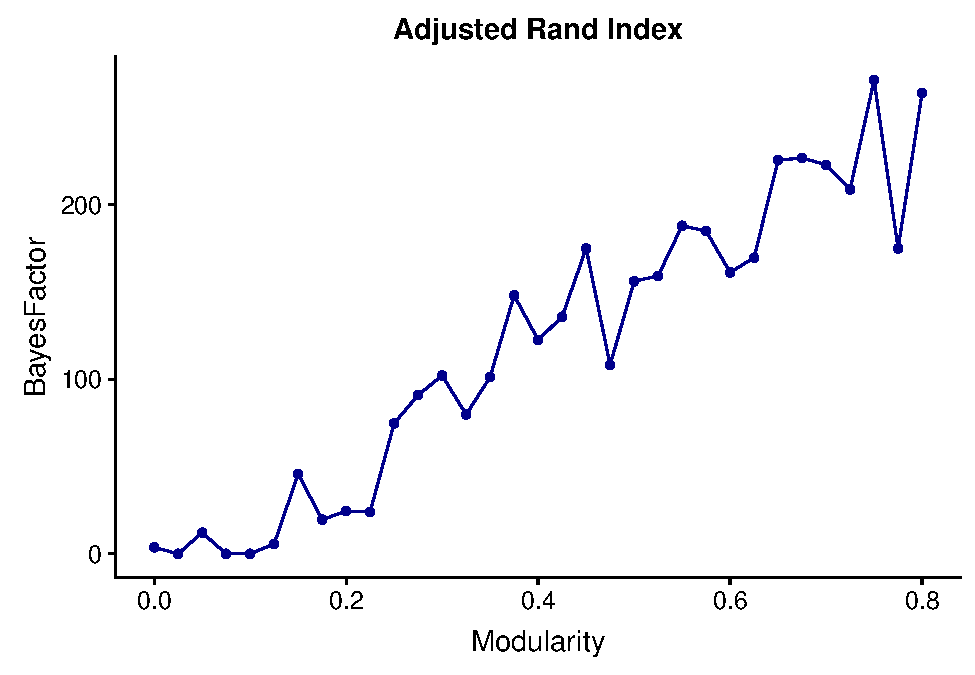
\includegraphics{Figure_Paper_files/figure-latex/unnamed-chunk-5-3.pdf}

\begin{Shaded}
\begin{Highlighting}[]
\NormalTok{####split join}
\NormalTok{BayesFactorVSModularitysplitjoin <-}\StringTok{ }\KeywordTok{read.csv}\NormalTok{(}\StringTok{"BayesFactorVSModularitysplitjoin.csv"}\NormalTok{)}

\NormalTok{df<-}\KeywordTok{data.frame}\NormalTok{(BayesFactorVSModularitysplitjoin}\OperatorTok{$}\NormalTok{BF,x)}
\KeywordTok{ggplot}\NormalTok{(}\DataTypeTok{data=}\NormalTok{df, }\KeywordTok{aes}\NormalTok{(}\DataTypeTok{x=}\NormalTok{x, }\DataTypeTok{y=}\NormalTok{BayesFactorVSModularitysplitjoin}\OperatorTok{$}\NormalTok{BF, }\DataTypeTok{group=}\DecValTok{1}\NormalTok{)) }\OperatorTok{+}
\StringTok{    }\KeywordTok{geom_line}\NormalTok{(}\DataTypeTok{color=}\StringTok{"dark blue"}\NormalTok{)}\OperatorTok{+}
\StringTok{    }\KeywordTok{geom_point}\NormalTok{(}\DataTypeTok{color=}\StringTok{"dark blue"}\NormalTok{)}\OperatorTok{+}
\StringTok{    }\KeywordTok{xlab}\NormalTok{(}\StringTok{"Modularity"}\NormalTok{) }\OperatorTok{+}
\StringTok{    }\KeywordTok{ylab}\NormalTok{(}\StringTok{"BayesFactor"}\NormalTok{) }\OperatorTok{+}
\StringTok{    }\KeywordTok{ggtitle}\NormalTok{(}\StringTok{"Split-join"}\NormalTok{)}
\end{Highlighting}
\end{Shaded}

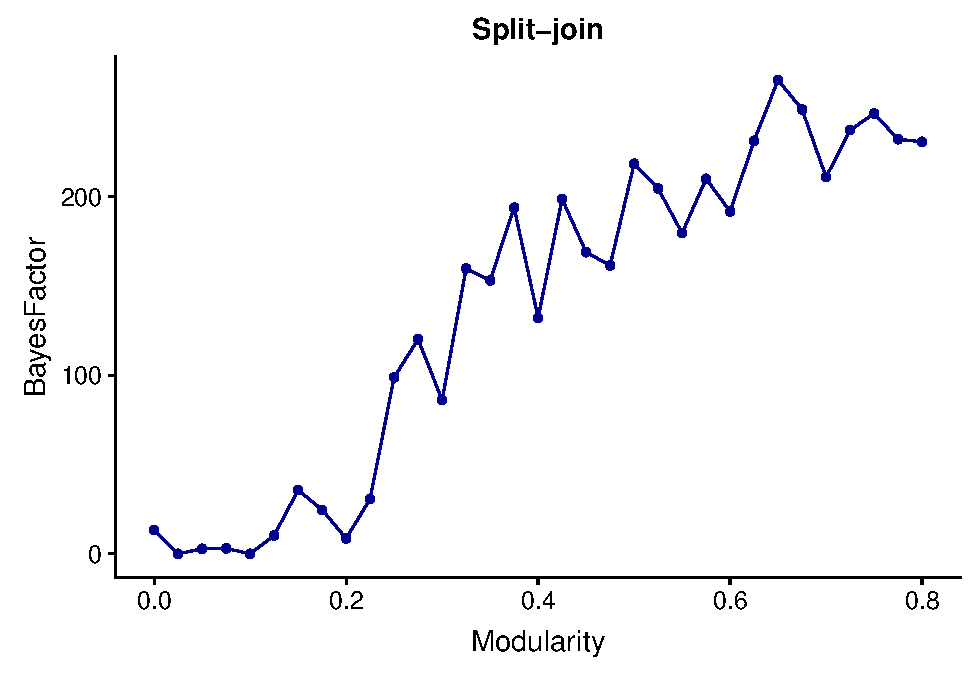
\includegraphics{Figure_Paper_files/figure-latex/unnamed-chunk-5-4.pdf}

\section{Fig.8 Dependent vs Independent
type}\label{fig.8-dependent-vs-independent-type}

\begin{Shaded}
\begin{Highlighting}[]
\CommentTok{#1}
\KeywordTok{setwd}\NormalTok{(}\StringTok{"/media/vpoli/MYFILES/CNR Tigem/Tutto per ROBIN/Dati/dati simulati"}\NormalTok{)}
\NormalTok{list.filenames<-}\KeywordTok{list.files}\NormalTok{(}\DataTypeTok{pattern=}\StringTok{".edgelist"}\NormalTok{)}
\NormalTok{BayesFactor<-}\OtherTok{NULL}
\ControlFlowTok{for}\NormalTok{ (i }\ControlFlowTok{in} \DecValTok{1}\OperatorTok{:}\KeywordTok{length}\NormalTok{(list.filenames))}
\NormalTok{\{}
\NormalTok{file <-}\StringTok{ }\NormalTok{list.filenames[i]}
\NormalTok{graph <-}\StringTok{ }\KeywordTok{prepGraph}\NormalTok{(file, }\DataTypeTok{header=}\OtherTok{FALSE}\NormalTok{) }
\NormalTok{graphRandom <-}\StringTok{ }\KeywordTok{random}\NormalTok{(graph)}
\NormalTok{Proc <-}\StringTok{ }\KeywordTok{robinRobust}\NormalTok{(}\DataTypeTok{graph=}\NormalTok{graph, }\DataTypeTok{graphRandom=}\NormalTok{graphRandom, }\DataTypeTok{measure=}\StringTok{"vi"}\NormalTok{, }
                  \DataTypeTok{method=}\StringTok{"louvain"}\NormalTok{, }\DataTypeTok{type=}\StringTok{"independent"}\NormalTok{)}

\NormalTok{BF<-}\KeywordTok{robinGPTest}\NormalTok{(}\DataTypeTok{ratio=}\NormalTok{Proc}\OperatorTok{$}\NormalTok{ratios)}
\NormalTok{df<-}\KeywordTok{data.frame}\NormalTok{(file,BF)}
\NormalTok{BayesFactor<-}\KeywordTok{rbind}\NormalTok{(BayesFactor,df)}
\NormalTok{\}}
\end{Highlighting}
\end{Shaded}

\begin{verbatim}
## [1] 502
## [1] 1004
## [1] 1506
## [1] 2008
## [1] 2510
## [1] 3012
## [1] 3514
## [1] 4016
## [1] 4518
## [1] 5020
## [1] 5522
## [1] 6024
##  Profile  1 
##  Profile  2 
## [1] 502
## [1] 1004
## [1] 1507
## [1] 2009
## [1] 2511
## [1] 3013
## [1] 3515
## [1] 4018
## [1] 4520
## [1] 5022
## [1] 5524
## [1] 6026
##  Profile  1 
##  Profile  2 
## [1] 502
## [1] 1004
## [1] 1507
## [1] 2009
## [1] 2511
## [1] 3014
## [1] 3516
## [1] 4018
## [1] 4520
## [1] 5022
## [1] 5525
## [1] 6027
##  Profile  1 
##  Profile  2 
## [1] 502
## [1] 1005
## [1] 1508
## [1] 2010
## [1] 2512
## [1] 3015
## [1] 3518
## [1] 4020
## [1] 4522
## [1] 5025
## [1] 5528
## [1] 6030
##  Profile  1 
##  Profile  2 
## [1] 502
## [1] 1004
## [1] 1507
## [1] 2009
## [1] 2511
## [1] 3013
## [1] 3515
## [1] 4018
## [1] 4520
## [1] 5022
## [1] 5524
## [1] 6026
##  Profile  1 
##  Profile  2 
## [1] 502
## [1] 1004
## [1] 1506
## [1] 2008
## [1] 2510
## [1] 3013
## [1] 3515
## [1] 4017
## [1] 4519
## [1] 5021
## [1] 5523
## [1] 6025
##  Profile  1 
##  Profile  2 
## [1] 503
## [1] 1005
## [1] 1508
## [1] 2010
## [1] 2513
## [1] 3016
## [1] 3518
## [1] 4021
## [1] 4523
## [1] 5026
## [1] 5529
## [1] 6031
##  Profile  1 
##  Profile  2 
## [1] 502
## [1] 1005
## [1] 1507
## [1] 2009
## [1] 2512
## [1] 3014
## [1] 3516
## [1] 4019
## [1] 4521
## [1] 5024
## [1] 5526
## [1] 6028
##  Profile  1 
##  Profile  2 
## [1] 502
## [1] 1004
## [1] 1505
## [1] 2007
## [1] 2509
## [1] 3011
## [1] 3513
## [1] 4014
## [1] 4516
## [1] 5018
## [1] 5520
## [1] 6022
##  Profile  1 
##  Profile  2 
## [1] 502
## [1] 1005
## [1] 1507
## [1] 2009
## [1] 2512
## [1] 3014
## [1] 3516
## [1] 4018
## [1] 4521
## [1] 5023
## [1] 5525
## [1] 6028
##  Profile  1 
##  Profile  2 
## [1] 502
## [1] 1004
## [1] 1506
## [1] 2008
## [1] 2510
## [1] 3012
## [1] 3514
## [1] 4016
## [1] 4518
## [1] 5020
## [1] 5523
## [1] 6025
##  Profile  1 
##  Profile  2 
## [1] 502
## [1] 1004
## [1] 1505
## [1] 2007
## [1] 2509
## [1] 3011
## [1] 3513
## [1] 4014
## [1] 4516
## [1] 5018
## [1] 5520
## [1] 6022
##  Profile  1 
##  Profile  2 
## [1] 502
## [1] 1004
## [1] 1506
## [1] 2008
## [1] 2510
## [1] 3013
## [1] 3515
## [1] 4017
## [1] 4519
## [1] 5021
## [1] 5523
## [1] 6025
##  Profile  1 
##  Profile  2 
## [1] 502
## [1] 1004
## [1] 1506
## [1] 2008
## [1] 2510
## [1] 3012
## [1] 3514
## [1] 4016
## [1] 4518
## [1] 5020
## [1] 5521
## [1] 6023
##  Profile  1 
##  Profile  2 
## [1] 502
## [1] 1005
## [1] 1507
## [1] 2010
## [1] 2512
## [1] 3015
## [1] 3517
## [1] 4020
## [1] 4522
## [1] 5024
## [1] 5527
## [1] 6029
##  Profile  1 
##  Profile  2 
## [1] 502
## [1] 1005
## [1] 1507
## [1] 2010
## [1] 2512
## [1] 3015
## [1] 3517
## [1] 4020
## [1] 4522
## [1] 5024
## [1] 5527
## [1] 6029
##  Profile  1 
##  Profile  2 
## [1] 502
## [1] 1005
## [1] 1507
## [1] 2010
## [1] 2512
## [1] 3014
## [1] 3517
## [1] 4019
## [1] 4522
## [1] 5024
## [1] 5526
## [1] 6029
##  Profile  1 
##  Profile  2 
## [1] 502
## [1] 1004
## [1] 1506
## [1] 2008
## [1] 2510
## [1] 3012
## [1] 3514
## [1] 4016
## [1] 4518
## [1] 5020
## [1] 5521
## [1] 6023
##  Profile  1 
##  Profile  2 
## [1] 502
## [1] 1004
## [1] 1506
## [1] 2009
## [1] 2511
## [1] 3013
## [1] 3515
## [1] 4017
## [1] 4519
## [1] 5022
## [1] 5524
## [1] 6026
##  Profile  1 
##  Profile  2 
## [1] 502
## [1] 1005
## [1] 1507
## [1] 2010
## [1] 2512
## [1] 3014
## [1] 3517
## [1] 4019
## [1] 4522
## [1] 5024
## [1] 5526
## [1] 6029
##  Profile  1 
##  Profile  2 
## [1] 502
## [1] 1004
## [1] 1506
## [1] 2008
## [1] 2510
## [1] 3012
## [1] 3514
## [1] 4016
## [1] 4518
## [1] 5020
## [1] 5523
## [1] 6025
##  Profile  1 
##  Profile  2 
## [1] 502
## [1] 1004
## [1] 1506
## [1] 2008
## [1] 2510
## [1] 3011
## [1] 3513
## [1] 4015
## [1] 4517
## [1] 5019
## [1] 5521
## [1] 6023
##  Profile  1 
##  Profile  2 
## [1] 502
## [1] 1004
## [1] 1506
## [1] 2009
## [1] 2511
## [1] 3013
## [1] 3515
## [1] 4017
## [1] 4519
## [1] 5022
## [1] 5524
## [1] 6026
##  Profile  1 
##  Profile  2 
## [1] 502
## [1] 1004
## [1] 1506
## [1] 2007
## [1] 2509
## [1] 3011
## [1] 3513
## [1] 4015
## [1] 4517
## [1] 5018
## [1] 5520
## [1] 6022
##  Profile  1 
##  Profile  2 
## [1] 502
## [1] 1003
## [1] 1504
## [1] 2006
## [1] 2508
## [1] 3009
## [1] 3510
## [1] 4012
## [1] 4514
## [1] 5015
## [1] 5516
## [1] 6018
##  Profile  1 
##  Profile  2 
## [1] 502
## [1] 1004
## [1] 1505
## [1] 2007
## [1] 2509
## [1] 3011
## [1] 3513
## [1] 4014
## [1] 4516
## [1] 5018
## [1] 5520
## [1] 6022
##  Profile  1 
##  Profile  2 
## [1] 502
## [1] 1004
## [1] 1506
## [1] 2008
## [1] 2510
## [1] 3013
## [1] 3515
## [1] 4017
## [1] 4519
## [1] 5021
## [1] 5523
## [1] 6025
##  Profile  1 
##  Profile  2 
## [1] 502
## [1] 1004
## [1] 1506
## [1] 2008
## [1] 2510
## [1] 3012
## [1] 3514
## [1] 4016
## [1] 4518
## [1] 5020
## [1] 5523
## [1] 6025
##  Profile  1 
##  Profile  2 
## [1] 502
## [1] 1004
## [1] 1506
## [1] 2008
## [1] 2510
## [1] 3012
## [1] 3514
## [1] 4016
## [1] 4518
## [1] 5020
## [1] 5521
## [1] 6023
##  Profile  1 
##  Profile  2 
## [1] 502
## [1] 1004
## [1] 1507
## [1] 2009
## [1] 2511
## [1] 3014
## [1] 3516
## [1] 4018
## [1] 4520
## [1] 5022
## [1] 5525
## [1] 6027
##  Profile  1 
##  Profile  2 
## [1] 502
## [1] 1004
## [1] 1506
## [1] 2009
## [1] 2511
## [1] 3013
## [1] 3515
## [1] 4017
## [1] 4519
## [1] 5022
## [1] 5524
## [1] 6026
##  Profile  1 
##  Profile  2 
## [1] 502
## [1] 1003
## [1] 1505
## [1] 2007
## [1] 2508
## [1] 3010
## [1] 3512
## [1] 4013
## [1] 4515
## [1] 5016
## [1] 5518
## [1] 6020
##  Profile  1 
##  Profile  2 
## [1] 502
## [1] 1004
## [1] 1505
## [1] 2007
## [1] 2509
## [1] 3010
## [1] 3512
## [1] 4014
## [1] 4516
## [1] 5018
## [1] 5519
## [1] 6021
##  Profile  1 
##  Profile  2
\end{verbatim}

\begin{Shaded}
\begin{Highlighting}[]
\KeywordTok{write.csv}\NormalTok{(BayesFactor,}\DataTypeTok{file=}\StringTok{"BayesFactorVSModularityIndependentLouvain.csv"}\NormalTok{)}

\NormalTok{BayesFactorVSModularity <-}\StringTok{ }\KeywordTok{read.csv}\NormalTok{(}\StringTok{"BayesFactorVSModularityIndependentLouvain.csv"}\NormalTok{)}
\NormalTok{x<-}\KeywordTok{seq}\NormalTok{(}\DecValTok{0}\NormalTok{,}\FloatTok{0.8}\NormalTok{,}\FloatTok{0.025}\NormalTok{)}
\NormalTok{df<-}\KeywordTok{data.frame}\NormalTok{(BayesFactorVSModularity,x)}
\KeywordTok{ggplot}\NormalTok{(}\DataTypeTok{data=}\NormalTok{df, }\KeywordTok{aes}\NormalTok{(}\DataTypeTok{x=}\NormalTok{x, }\DataTypeTok{y=}\NormalTok{BF, }\DataTypeTok{group=}\DecValTok{1}\NormalTok{)) }\OperatorTok{+}
\StringTok{    }\KeywordTok{geom_line}\NormalTok{(}\DataTypeTok{color=}\StringTok{"dark blue"}\NormalTok{)}\OperatorTok{+}
\StringTok{    }\KeywordTok{xlab}\NormalTok{(}\StringTok{"Modularity"}\NormalTok{) }\OperatorTok{+}
\StringTok{    }\KeywordTok{ylab}\NormalTok{(}\StringTok{"BayesFactor"}\NormalTok{) }\OperatorTok{+}
\StringTok{    }\KeywordTok{ggtitle}\NormalTok{(}\StringTok{"Independent"}\NormalTok{)}
\end{Highlighting}
\end{Shaded}

\includegraphics{Figure_Paper_files/figure-latex/unnamed-chunk-6-1.pdf}

\begin{Shaded}
\begin{Highlighting}[]
\CommentTok{#2}
\KeywordTok{setwd}\NormalTok{(}\StringTok{"/media/vpoli/MYFILES/CNR Tigem/Tutto per ROBIN/Dati/dati simulati"}\NormalTok{)}
\NormalTok{list.filenames<-}\KeywordTok{list.files}\NormalTok{(}\DataTypeTok{pattern=}\StringTok{".edgelist"}\NormalTok{)}
\NormalTok{BayesFactor<-}\OtherTok{NULL}
\ControlFlowTok{for}\NormalTok{ (i }\ControlFlowTok{in} \DecValTok{1}\OperatorTok{:}\KeywordTok{length}\NormalTok{(list.filenames))}
\NormalTok{\{}
\NormalTok{file <-}\StringTok{ }\NormalTok{list.filenames[i]}
\NormalTok{graph <-}\StringTok{ }\KeywordTok{prepGraph}\NormalTok{(file, }\DataTypeTok{header=}\OtherTok{FALSE}\NormalTok{) }
\NormalTok{graphRandom <-}\StringTok{ }\KeywordTok{random}\NormalTok{(graph)}
\NormalTok{Proc <-}\StringTok{ }\KeywordTok{robinRobust}\NormalTok{(}\DataTypeTok{graph=}\NormalTok{graph, }\DataTypeTok{graphRandom=}\NormalTok{graphRandom, }\DataTypeTok{measure=}\StringTok{"vi"}\NormalTok{, }
                  \DataTypeTok{method=}\StringTok{"louvain"}\NormalTok{, }\DataTypeTok{type=}\StringTok{"dependent"}\NormalTok{)}

\NormalTok{BF<-}\KeywordTok{robinGPTest}\NormalTok{(}\DataTypeTok{ratio=}\NormalTok{Proc}\OperatorTok{$}\NormalTok{ratios)}
\NormalTok{df<-}\KeywordTok{data.frame}\NormalTok{(file,BF)}
\NormalTok{BayesFactor<-}\KeywordTok{rbind}\NormalTok{(BayesFactor,df)}
\NormalTok{\}}
\end{Highlighting}
\end{Shaded}

\begin{verbatim}
## [1] 9188
## [1] 8369
## [1] 7541
## [1] 6748
## [1] 5959
## [1] 5173
## [1] 4412
## [1] 3651
## [1] 2956
## [1] 2330
## [1] 1700
## [1] 1154
##  Profile  1 
##  Profile  2 
## [1] 9218
## [1] 8375
## [1] 7552
## [1] 6736
## [1] 5954
## [1] 5171
## [1] 4390
## [1] 3677
## [1] 2984
## [1] 2350
## [1] 1743
## [1] 1232
##  Profile  1 
##  Profile  2 
## [1] 9183
## [1] 8346
## [1] 7523
## [1] 6707
## [1] 5927
## [1] 5129
## [1] 4400
## [1] 3661
## [1] 2942
## [1] 2279
## [1] 1681
## [1] 1148
##  Profile  1 
##  Profile  2 
## [1] 9201
## [1] 8354
## [1] 7508
## [1] 6682
## [1] 5888
## [1] 5098
## [1] 4331
## [1] 3581
## [1] 2889
## [1] 2262
## [1] 1663
## [1] 1144
##  Profile  1 
##  Profile  2 
## [1] 9200
## [1] 8363
## [1] 7530
## [1] 6715
## [1] 5915
## [1] 5127
## [1] 4367
## [1] 3598
## [1] 2904
## [1] 2245
## [1] 1669
## [1] 1143
##  Profile  1 
##  Profile  2 
## [1] 9207
## [1] 8375
## [1] 7540
## [1] 6711
## [1] 5893
## [1] 5098
## [1] 4328
## [1] 3584
## [1] 2882
## [1] 2228
## [1] 1642
## [1] 1120
##  Profile  1 
##  Profile  2 
## [1] 9203
## [1] 8354
## [1] 7520
## [1] 6728
## [1] 5919
## [1] 5143
## [1] 4399
## [1] 3640
## [1] 2930
## [1] 2276
## [1] 1678
## [1] 1170
##  Profile  1 
##  Profile  2 
## [1] 9198
## [1] 8369
## [1] 7547
## [1] 6735
## [1] 5931
## [1] 5145
## [1] 4371
## [1] 3635
## [1] 2966
## [1] 2313
## [1] 1722
## [1] 1208
##  Profile  1 
##  Profile  2 
## [1] 9192
## [1] 8370
## [1] 7544
## [1] 6734
## [1] 5942
## [1] 5165
## [1] 4391
## [1] 3663
## [1] 2963
## [1] 2304
## [1] 1676
## [1] 1169
##  Profile  1 
##  Profile  2 
## [1] 9202
## [1] 8376
## [1] 7547
## [1] 6741
## [1] 5936
## [1] 5153
## [1] 4422
## [1] 3680
## [1] 2959
## [1] 2310
## [1] 1683
## [1] 1150
##  Profile  1 
##  Profile  2 
## [1] 9193
## [1] 8373
## [1] 7545
## [1] 6744
## [1] 5960
## [1] 5177
## [1] 4411
## [1] 3669
## [1] 2948
## [1] 2314
## [1] 1727
## [1] 1205
##  Profile  1 
##  Profile  2 
## [1] 9188
## [1] 8373
## [1] 7554
## [1] 6739
## [1] 5926
## [1] 5139
## [1] 4374
## [1] 3644
## [1] 2933
## [1] 2265
## [1] 1681
## [1] 1149
##  Profile  1 
##  Profile  2 
## [1] 9206
## [1] 8362
## [1] 7528
## [1] 6716
## [1] 5905
## [1] 5121
## [1] 4360
## [1] 3634
## [1] 2898
## [1] 2229
## [1] 1627
## [1] 1083
##  Profile  1 
##  Profile  2 
## [1] 9179
## [1] 8320
## [1] 7479
## [1] 6677
## [1] 5873
## [1] 5087
## [1] 4327
## [1] 3581
## [1] 2883
## [1] 2222
## [1] 1638
## [1] 1125
##  Profile  1 
##  Profile  2 
## [1] 9211
## [1] 8376
## [1] 7544
## [1] 6746
## [1] 5946
## [1] 5158
## [1] 4399
## [1] 3667
## [1] 2958
## [1] 2337
## [1] 1755
## [1] 1234
##  Profile  1 
##  Profile  2 
## [1] 9207
## [1] 8375
## [1] 7557
## [1] 6737
## [1] 5939
## [1] 5172
## [1] 4393
## [1] 3685
## [1] 2991
## [1] 2328
## [1] 1720
## [1] 1176
##  Profile  1 
##  Profile  2 
## [1] 9193
## [1] 8353
## [1] 7546
## [1] 6718
## [1] 5910
## [1] 5114
## [1] 4348
## [1] 3625
## [1] 2941
## [1] 2278
## [1] 1688
## [1] 1165
##  Profile  1 
##  Profile  2 
## [1] 9186
## [1] 8352
## [1] 7533
## [1] 6719
## [1] 5934
## [1] 5132
## [1] 4388
## [1] 3660
## [1] 2961
## [1] 2331
## [1] 1707
## [1] 1169
##  Profile  1 
##  Profile  2 
## [1] 9209
## [1] 8385
## [1] 7586
## [1] 6756
## [1] 5989
## [1] 5196
## [1] 4428
## [1] 3696
## [1] 3007
## [1] 2352
## [1] 1749
## [1] 1205
##  Profile  1 
##  Profile  2 
## [1] 9198
## [1] 8347
## [1] 7509
## [1] 6721
## [1] 5933
## [1] 5164
## [1] 4408
## [1] 3694
## [1] 3008
## [1] 2362
## [1] 1750
## [1] 1213
##  Profile  1 
##  Profile  2 
## [1] 9207
## [1] 8378
## [1] 7549
## [1] 6737
## [1] 5954
## [1] 5154
## [1] 4394
## [1] 3648
## [1] 2942
## [1] 2303
## [1] 1709
## [1] 1183
##  Profile  1 
##  Profile  2 
## [1] 9194
## [1] 8357
## [1] 7540
## [1] 6722
## [1] 5961
## [1] 5187
## [1] 4428
## [1] 3693
## [1] 3000
## [1] 2343
## [1] 1736
## [1] 1234
##  Profile  1 
##  Profile  2 
## [1] 9204
## [1] 8365
## [1] 7540
## [1] 6732
## [1] 5928
## [1] 5141
## [1] 4373
## [1] 3673
## [1] 2964
## [1] 2311
## [1] 1702
## [1] 1187
##  Profile  1 
##  Profile  2 
## [1] 9203
## [1] 8348
## [1] 7525
## [1] 6714
## [1] 5887
## [1] 5100
## [1] 4337
## [1] 3595
## [1] 2906
## [1] 2256
## [1] 1670
## [1] 1158
##  Profile  1 
##  Profile  2 
## [1] 9194
## [1] 8348
## [1] 7525
## [1] 6712
## [1] 5910
## [1] 5116
## [1] 4366
## [1] 3651
## [1] 2922
## [1] 2282
## [1] 1669
## [1] 1159
##  Profile  1 
##  Profile  2 
## [1] 9175
## [1] 8309
## [1] 7487
## [1] 6673
## [1] 5893
## [1] 5129
## [1] 4364
## [1] 3636
## [1] 2941
## [1] 2275
## [1] 1679
## [1] 1161
##  Profile  1 
##  Profile  2 
## [1] 9200
## [1] 8351
## [1] 7508
## [1] 6690
## [1] 5900
## [1] 5118
## [1] 4364
## [1] 3626
## [1] 2911
## [1] 2269
## [1] 1671
## [1] 1150
##  Profile  1 
##  Profile  2 
## [1] 9208
## [1] 8352
## [1] 7527
## [1] 6695
## [1] 5898
## [1] 5120
## [1] 4361
## [1] 3618
## [1] 2908
## [1] 2265
## [1] 1655
## [1] 1127
##  Profile  1 
##  Profile  2 
## [1] 9188
## [1] 8367
## [1] 7548
## [1] 6714
## [1] 5910
## [1] 5112
## [1] 4342
## [1] 3604
## [1] 2904
## [1] 2264
## [1] 1663
## [1] 1151
##  Profile  1 
##  Profile  2 
## [1] 9190
## [1] 8350
## [1] 7528
## [1] 6729
## [1] 5932
## [1] 5148
## [1] 4374
## [1] 3672
## [1] 2975
## [1] 2324
## [1] 1733
## [1] 1193
##  Profile  1 
##  Profile  2 
## [1] 9196
## [1] 8372
## [1] 7553
## [1] 6727
## [1] 5930
## [1] 5156
## [1] 4404
## [1] 3668
## [1] 2983
## [1] 2300
## [1] 1709
## [1] 1181
##  Profile  1 
##  Profile  2 
## [1] 9189
## [1] 8350
## [1] 7511
## [1] 6670
## [1] 5864
## [1] 5065
## [1] 4300
## [1] 3562
## [1] 2859
## [1] 2225
## [1] 1636
## [1] 1115
##  Profile  1 
##  Profile  2 
## [1] 9179
## [1] 8335
## [1] 7509
## [1] 6701
## [1] 5903
## [1] 5134
## [1] 4384
## [1] 3643
## [1] 2937
## [1] 2281
## [1] 1691
## [1] 1179
##  Profile  1 
##  Profile  2
\end{verbatim}

\begin{Shaded}
\begin{Highlighting}[]
\KeywordTok{write.csv}\NormalTok{(BayesFactor,}\DataTypeTok{file=}\StringTok{"BayesFactorVSModularityDependentLouvain.csv"}\NormalTok{)}

\NormalTok{BayesFactorVSModularity <-}\StringTok{ }\KeywordTok{read.csv}\NormalTok{(}\StringTok{"BayesFactorVSModularityDependentLouvain.csv"}\NormalTok{)}
\NormalTok{x<-}\KeywordTok{seq}\NormalTok{(}\DecValTok{0}\NormalTok{,}\FloatTok{0.8}\NormalTok{,}\FloatTok{0.025}\NormalTok{)}
\NormalTok{df<-}\KeywordTok{data.frame}\NormalTok{(BayesFactorVSModularity,x)}
\KeywordTok{ggplot}\NormalTok{(}\DataTypeTok{data=}\NormalTok{df, }\KeywordTok{aes}\NormalTok{(}\DataTypeTok{x=}\NormalTok{x, }\DataTypeTok{y=}\NormalTok{BF, }\DataTypeTok{group=}\DecValTok{1}\NormalTok{)) }\OperatorTok{+}
\StringTok{    }\KeywordTok{geom_line}\NormalTok{(}\DataTypeTok{color=}\StringTok{"dark blue"}\NormalTok{)}\OperatorTok{+}
\StringTok{    }\KeywordTok{xlab}\NormalTok{(}\StringTok{"Modularity"}\NormalTok{) }\OperatorTok{+}
\StringTok{    }\KeywordTok{ylab}\NormalTok{(}\StringTok{"BayesFactor"}\NormalTok{) }\OperatorTok{+}
\StringTok{    }\KeywordTok{ggtitle}\NormalTok{(}\StringTok{"Dependent"}\NormalTok{)}
\end{Highlighting}
\end{Shaded}

\includegraphics{Figure_Paper_files/figure-latex/unnamed-chunk-6-2.pdf}


\end{document}
